%------------------------------------------------------------------------------%
%                                                                              %
%                                                                              %
%   EnsiRapport Template                                                       %
%                                                                              %
%   Version : 1.0                                                              %
%                                                                              %
%------------------------------------------------------------------------------%



\documentclass[liens,entete-ensimag,margeCorrection,onecolumn,12pt]{ensirapport}
% options possibles:
% -  ('10pt', '11pt' and '12pt') taille de police.
% -  ('a4paper', 'letterpaper', 'a5paper', 'legalpaper', 'executivepaper' and 'landscape') taille de papier.
% -  ('sans' and 'roman') famille de police.
% -- ('liens') ajoute les liens dans le sommaire.
% -- ('entete,entete-ensimag') ajoute des belles entetes avec logo ensimag ou pas.
% -- ('margeCorrection') diminue les enormes marges de latex.
% -- ('minted') inclus minted pour colorer les codes sources, ne fonctionne pas à l'ensimag.
% -  ('onecolumn','twocolumn') une ou deux colonnes
% -  ('fleqn','leqno') formules mathématique alignées a gauche ou a droite.
% -  ('notitlepage','titlepage') sans ou avec page de garde pour le titre


\usepackage{titling} % Allows custom title configuration
\usepackage{dirtree}
\usepackage{indentfirst}
\usepackage{listings}
\usepackage{float}
\usepackage{enumitem}
\usepackage[title,titletoc,toc,page]{appendix}
\usepackage[toc,section=section]{glossaries}

\usepackage{color}
\definecolor{editorGray}{rgb}{0.95, 0.95, 0.95}
\definecolor{editorOcher}{rgb}{1, 0.5, 0} % #FF7F00 -> rgb(239, 169, 0)
\definecolor{editorGreen}{rgb}{0, 0.5, 0} % #007C00 -> rgb(0, 124, 0)
\usepackage{upquote}
\usepackage{listings}
\usepackage{pdfpages}
\usepackage{fancybox}
\usepackage[T1]{fontenc}
\usepackage{lmodern}
\usepackage{titlesec}
\usepackage[nottoc, notlof, notlot]{tocbibind}
\usepackage{babel}
\usepackage{float}
%\usepackage{parskip}
\setlength{\parindent}{0pt}

%\titlespacing\section{0pt}{12pt plus 4pt minus 2pt}{0pt plus 2pt minus 2pt}
%\titlespacing\subsection{0pt}{12pt plus 4pt minus 2pt}{0pt plus 2pt minus 2pt}
%\titlespacing\subsubsection{0pt}{12pt plus 4pt minus 2pt}{0pt plus 2pt minus 2pt}
%\titlespacing\paragraph{0pt}{0pt plus 4pt minus 2pt}{0pt plus 2pt minus 2pt} % titlesec
%\titlespacing\subparagraph{0pt}{0pt plus 4pt minus 2pt}{0pt plus 2pt minus 2pt} % titlesec

% \titlespacing*{<command>}{<left>}{<before-sep>}{<after-sep>}

%\titlespacing{\paragraph}{0pt}{10pt}{10pt} % titlesec

\titlespacing{\subparagraph}{20pt}{3.5ex plus 1ex minus .2ex}{0ex plus .0ex}
\titleformat{\subparagraph}  {\normalfont\fontsize{0.85em}{0.7em}\bfseries}  {\thesubparagraph}{1em}{}

% Change Name of Table of Contents 
\renewcommand\contentsname{Table of Contents}
\addto\captionsenglish{%
	\renewcommand{\contentsname}{Table des matières}%\\
}

\addto\captionsenglish{\renewcommand\listfigurename{Liste des figures}}


% Change Name of Appendices
\renewcommand\appendixtocname{Annexes}
\renewcommand\appendixname{Annexes}
\renewcommand\appendixpagename{Annexes}
%\usepackage{paralist}
%\renewenvironment{itemize}[1]{\begin{compactitem}#1}{\end{compactitem}}
%\renewenvironment{enumerate}[1]{\begin{compactenum}#1}{\end{compactenum}}
%\renewenvironment{description}[0]{\begin{compactdesc}}{\end{compactdesc}}
%\setlist[enumerate]{itemsep=0mm}

%    \makeatletter
%    \renewcommand\paragraph{\@startsection{paragraph}{4}{\z@}%
%                                         {-3.25ex\@plus -1ex \@minus -.2ex}%
%                                         {0.0001pt \@plus .2ex}%
%                                         {\normalfont\normalsize\bfseries}}
%    \renewcommand\subparagraph{\@startsection{subparagraph}{5}{\z@}%
%                                         {-3.25ex\@plus -1ex \@minus -.2ex}%
%                                         {0.0001pt \@plus .2ex}%
%                                         {\normalfont\normalsize\bfseries}}
%    \makeatother

\newenvironment{sitemize}
{ \begin{itemize}
    \setlength{\itemsep}{0pt}
    \setlength{\parskip}{0pt}
    \setlength{\parsep}{0pt}     }
{ \end{itemize}                  } 

\lstdefinelanguage{JavaScript}{
  morekeywords={typeof, new, true, false, catch, function, return, null, catch, switch, var, if, in, while, do, else, case, break},
  morecomment=[s]{/*}{*/},
  morecomment=[l]//,
  morestring=[b]",
  morestring=[b]'
}

\lstdefinelanguage{HTML5}{
        language=html,
        sensitive=true,
        alsoletter={<>=-},
        otherkeywords={
        % HTML tags
        <html>, <head>, <title>, </title>, <meta, />, </head>, <body>,
        <canvas, \/canvas>, <script>, </script>, </body>, </html>, <!, html>, <style>, </style>, ><
        },
        ndkeywords={
        % General
        =,
        % HTML attributes
        charset=, id=, width=, height=,
        % CSS properties
        border:, transform:, -moz-transform:, transition-duration:, transition-property:, transition-timing-function:
        },
        morecomment=[s]{<!--}{-->},
        tag=[s]
}

\lstset{%
    % Basic design
    backgroundcolor=\color{editorGray},
    basicstyle={\small\ttfamily},
    frame=l,
    % Line numbers
    xleftmargin={0.75cm},
    numbers=left,
    stepnumber=1,
    firstnumber=1,
    numberfirstline=true,
    % Code design
    keywordstyle=\color{blue}\bfseries,
    commentstyle=\color{darkgray}\ttfamily,
    ndkeywordstyle=\color{editorGreen}\bfseries,
    stringstyle=\color{editorOcher},
    % Code
    language=HTML5,
    alsolanguage=JavaScript,
    alsodigit={.:;},
    tabsize=2,
    showtabs=false,
    showspaces=false,
    showstringspaces=false,
    extendedchars=true,
    breaklines=true,
    % Support for German umlauts
    literate=%
    {Ö}{{\"O}}1
    {Ä}{{\"A}}1
    {Ü}{{\"U}}1
    {ß}{{\ss}}1
    {ü}{{\"u}}1
    {ä}{{\"a}}1
    {ö}{{\"o}}1
}

% Correct the default ugly font of the lstlistings 
\lstset{basicstyle=\ttfamily\small,breaklines=true}

% ``\Listing{...}'' command typesets its argument as a code block -
% with monospace font and whitespace preserved.  It is an
% environment-like command accepting multiple paragraphs.
\def\Listing{\bigskip\begingroup%
\setlength{\parskip}{0pc}\addtolength{\parindent}{1pc}%
\tt\scriptsize\obeylines\obeyspaces\PreserveWhitespace\ListingBody}

% ``\ListingBody'' is an auxillary command need to make Listing work.
% It inserts the argument and closes the group opened by Listing.
\long\def\ListingBody#1{#1\endgroup\smallskip}

% \PreserveWhitespace makes leading spaces appear as-is.  To make
% leading spaces appear, we have to set space to be an active
% character that exands to a non-breakable space.  The command for
% this is ``\let =\ ``, but unfortunately lifting this command to a
% macro does not quite work because space is not active during the
% definition of the macro - it needs to be made active using
% ``\catcode''.  Therefore we define our macro in a little block of
% code where space is made active:
\begingroup
\catcode32=\active
\gdef\PreserveWhitespace{\catcode32=\active\let =\ }
\endgroup

\newcommand{\HorRule}{ \rule{\linewidth}{0pt}} % Defines the gold horizontal rule around the title

\pretitle{
  \vspace{-2cm}
  \hspace{-1cm}
  
\includegraphics[height=70pt]{img/supralog.jpg}
  \hfill
  
\includegraphics[height=85pt]{ensilogo.png}
  \vfill

  \begin{center}\fontsize{14}{14} \usefont{OT1}{cmr}{}{n}
  Grenoble INP - ENSIMAG \\
École nationale supérieure d'informatique et de mathématiques appliquées de Grenoble
  \end{center}
\vspace{2cm}

\begin{center}\HorRule \fontsize{25}{25} \usefont{OT1}{cmr}{}{n}  \selectfont

  

} % Horizontal rule before the title

\posttitle{\par\end{center}
  \begin{center}\fontsize{14}{14} \usefont{OT1}{cmr}{}{n}
  Effectué chez Supralog
  \end{center}
  
  \vspace{1.5cm}

  \begin{center}
    \shadowbox{
	\begin{minipage}{0.9\textwidth}
	\vspace{0.3cm}
	\begin{center}\fontsize{12}{12} \usefont{OT1}{cmr}{}{n}
	{\Huge Architecture et Développement Java Backend pour une Solution E-Santé}\\~
	\end{center}
	\end{minipage}
	}
  \end{center}


%  \begin{flushright}
%    \small $22^{rd}$ June -- $4^{th}$ September.
%  \end{flushright}

\vskip 2cm
} % Whitespace under the title

\preauthor{
  %\begin{center}
  %\includegraphics[height=2cm]{img/logo_idevicecloud}\\
  %\vspace{0.2cm}
  %\bf
  %Design and development of a 3D graphical interfaces representing a calculation scheme
  %deployed on the nodes of the mesh iDeviceCloud
  %\vspace{0.2cm}
  %\end{center}



  \begin{center}\fontsize{13}{13} \lineskip 0.5em \usefont{OT1}{cmr}{}{sl}
  } % Author font configuration


  \postauthor{\footnotesize  % Configuration for the institution name
  \begin{center}\fontsize{13}{13} \usefont{OT1}{cmr}{}{n}
  	$3A$ $-$ Filière Ingénierie des systèmes d'information\
    
    \vspace{0.5cm}
	29 Février 2016 - 26 Août 2016
  \end{center}
    \date{} % Add a date here if you would like one to appear underneath the title block

	\vskip 1.5cm
	\begin{center}\fontsize{13}{13} \usefont{OT1}{cmr}{}{n}
    \begin{tabular*}{\textwidth }{@{\extracolsep{\fill}} l l}
      \textbf{Supralog}                & \textbf{Responsable de stage}\\
      {\footnotesize Immeuble Le Chorus} & ~~~Nicolas \textsc{THIBAULT}\\
      {\footnotesize 2203, Chemin de Saint-Claude} & \textbf{Tuteur de l'école}\\
      {\footnotesize 06600 ANTIBES}                 & ~~~Sylvain \textsc{BOUVERET}\\
    \end{tabular*}
	\end{center}
\par\end{center}\HorRule} % Horizontal rule after the title

% Glossaire 
\makenoidxglossaries
\defglsentryfmt[main]{\glsgenentryfmt{}{}{*}}

\newglossaryentry{ARL}{
	name=ARL,
	description={est l'acronyme de "Accusé de Réception Logique".}
}

\newglossaryentry{CPS}{
	name=CPS,
	description={est l'acronyme de "Cartes Professionnelles de Santé".}
}

\newglossaryentry{Sesam Vitale}{
  name=Sesam Vitale,
  description={Le programme SESAM-Vitale est un programme de dématérialisation des feuilles de soins pour l'assurance maladie en France, qui repose sur la carte Vitale.}
}

\newglossaryentry{Topaze Maestro}{
  name=Topaze Maestro,
  description={est l'une des versions ressente du progiciel d'e-santé actuellement commercialisé par Supralog. Le logiciel fonctionne comme une application de bureau pour Windows.}
}

\newglossaryentry{Topaze Web}{
  name=Topaze Web,
  description={est la refonte web de Topaze Maestro.}
}

\newglossaryentry{SAAS}{
  name=SAAS,
  description={"Software As A Service" ou logiciel en tant que service. Il s'agit d'un business modèle visant à vendre des accès à une application qui tourne sur un serveur, plutôt que de vendre le logiciel comme un produit.}
}

\newglossaryentry{IDLOG}{
  name=IDLOG,
  description={est un groupe familial créé en 2002 afin de regrouper les sociétés SUPRALOG et IDEA.}
}

\newglossaryentry{IDEA}{
  name=IDEA,
  description={est la société créée en 1987 qui est responsable de la commercialisation de Topaze.}
}

\newglossaryentry{SUPRALOG}{
  name=SUPRALOG,
  description={est la société fondée en 1997 qui a créé le progiciel d'e-santé Topaze.}
}


\newglossaryentry{OLE}{
  name=OLE,
  description={est l'acronyme de "Object Linking and Embedding". Il s'agit d'un protocole développé par Microsoft permettant de faire de la liaison dynamique d'objets dans Windows.}
}

\newglossaryentry{RTF}{
  name=RTF,
  description={est l'acronyme de "Rich Text Format". Il s'agit d'un format de fichier développé par Microsoft et utilisable dans la plupart des éditeurs de textes.}
}

\newglossaryentry{FSE}{
  name=FSE,
  description={est l'acronyme de "Feuille de Soins Électronique". Il s'agit du document envoyé à la caisse, pour remboursement.}
}

\newglossaryentry{DRE}{
	name=DRE,
	description={est l'acronyme de "Demande de Remboursement Électronique". Il s'agit du document envoyé à la complémentaire, pour remboursement.}
}

\newglossaryentry{DAP}{
	name=DAP,
	description={est l'acronyme de "Demande d'Accord Préalable". Les DAP concernent les rééducations en masso-kinésithérapie. Pour chaque type de rééducations, il est prévu qu'un certain nombre de séances soient remboursées par la sécurité sociale. Si ce nombre de séances doit être dépassé, il convient de faire une demande préalable (la DAP).}
}

\newglossaryentry{DSI}{
	name=DSI,
	description={est l'acronyme de "Démarche de Soin Infirmier".}
}

\newglossaryentry{ORM}{
  name=ORM,
  description={est l'acronyme de "Object-relational mapping". Il s'agit d'une technique permettant de manipuler les données de la base de données comme s'il s'agissait d'objets.}
}

\newglossaryentry{SCOR}{
	name=SCOR,
	description={est l'acronyme de "SCannérisation des ORdonnances".}
}

\newglossaryentry{WYSIWYG}{
  name=WYSIWYG,
  description={est l'acronyme de "What You See Is What You Get". Cela désigne le plus souvent un éditeur graphique qui produit le code de ce qui est affiché à l'écran.}
}



\begin{document}

\title{Rapport de Projet de Fin d'Etudes}
\author{Alexandre Rupp}
\date{}

% Page de garde
 \pagenumbering{gobble} 
	\maketitle
 \thispagestyle{empty}
 
 
\newpage
\thispagestyle{fancy}
\pagenumbering{arabic}  

% Coordonnées TODO
%\newpage
\section*{Contacts}

\paragraph{Nicolas Thibault (Tuteur de la structure d'accueil)}

\begin{sitemize}
\item \textbf{Adresse :}  \\

SUPRALOG \\
Immeuble Le Chorus\\
2203, Chemin de Saint Claude\\
06600 Antibes \\
FRANCE \\

\item \textbf{Email :} nthibault@supralog.com
\end{sitemize}

\paragraph{Sylvain Bouveret (Tuteur de l'école)}

\begin{sitemize}
\item \textbf{Adresse :}  \\

Bureau D301 bis, \\
Bâtiment D 681, \\
rue de la Passerelle. \\
BP 72. F-38402 SAINT-MARTIN-D'HÈRES. \\
FRANCE.\\

\item \textbf{Email :} sylvain.bouveret@imag.fr
\end{sitemize}

\paragraph{Alexandre Rupp (Stagiaire)}
\begin{sitemize}
\item \textbf{Adresse :}  \\

Appt 4201 \\
Les callades de Sophia \\
475 rue Evariste Galois \\
Sophia Antipolis \\
06560 Valbonne \\
FRANCE\\

\item \textbf{Téléphone :} 06 13 80 34 87

\item \textbf{Email :} alexandre.rupp@ensimag.grenoble-inp.fr
\end{sitemize}  
\newpage
\section*{Remerciements}

Je tiens à remercier les personnes qui ont permis le bon déroulement de ce stage : \\

Tout d'abord, je tiens à remercier mon maitre de stage, M. Nicolas Thibault, directeur technique de Supralog, pour sa confiance, son support et les tâches intéressantes qu'il m'a confiées.\\

Ensuite, je tiens à remercier M. Philippe Salvan, directeur de Supralog, pour m'avoir accueilli dans son entreprise.\\

Je tiens ensuite à remercier les membres de l'équipe Topaze Web pour leur disponibilité, leur bonne humeur au quotidien et en particulier M. El Jaï qui m'a beaucoup aidé et a partagé avec moi son expertise en Java.\\

Je remercie également Dr. Sylvain Bouveret, mon tuteur à l'Ensimag, pour son suivi et ses conseils lors de la rédaction de ce rapport.\\

Enfin, je remercie tous les membres de Supralog qui m'ont permis de réaliser ce stage dans les meilleures conditions.


% Table des matières 
\newpage
\addtocontents{toc}{\protect\enlargethispage{5mm}}
\clearpage
\vspace*{-47pt}
\tableofcontents

% Table des figures 
\newpage
\listoffigures

% Résumé (1 page) TODO
\newpage
\section*{Résumé}  

Dans le cadre de ma dernière année d'école d'ingénieurs à l’Ensimag, j’ai réalisé mon projet de fin d’études d’une durée de six mois au sein de l’entreprise Supralog.\\

Le but du projet était de participer à la conception et au développement d’une application web d’e-santé à destination des cabinets médicaux. Cette application réalisée en Java, Spring et JSF selon une architecture 3-Tiers est la refonte d'un logiciel plus ancien qui est distribué en tant qu'application de bureau pour Windows. Le logiciel permet entre autres de gérer les feuilles de soins électroniques, la facturation, l'activité d'un cabinet et utilise la technologie \textit{\gls{Sesam Vitale}}.\\
%legacy

Dans ce cadre, j’ai eu à réaliser le dossier médical d'un patient et les différentes fonctionnalités permettant de le gérer. Pour ce faire, j'ai d'abord fait un état des lieux des fonctionnalités présentes dans le logiciel d'origine, puis j'ai analysé l'existant sur la nouvelle application et j'ai conçu et implémenté une solution qui puisse s'y greffer.\\

Finalement, ce stage m'a permis de développer mes compétences sur les technologies \gls{HTML5}, \gls{CSS3}, \gls{JavaScript}, \gls{Java 8}, \gls{Java EE}, \gls{JSF}, \gls{Spring} (\gls{IOC}, \gls{AOP}, \gls{MVC}) et \gls{Hibernate}. J'ai  travaillé au sein d'une équipe qui applique les méthodes agiles et sur un projet qui utilise l'intégration continue. Enfin, cela m'a donné l'occasion de découvrir les aspects métiers liés aux prescriptions médicales, aux feuilles de soins et à l'assurance maladie.\\

\textbf{Mots-clé}: Java, JSF, Spring, Hibernate, e-santé, Architecture 3-Tiers, Sesam Vitale.

% Glossaire
\newpage
\printnoidxglossary[title={Glossaire}]

 
\newcommand{\lc}{\cellcolor{blue!60}}
\renewcommand{\arraystretch}{1.3}

% Content :

\newpage
\section{Introduction} % (2-3 ¶) Problématique + objectifs + plan  

Ce rapport fait état du travail réalisé durant mon stage de six mois chez \textit{Supralog}.\\

Historiquement, \textit{Supralog} est la société éditrice du logiciel \textit{\gls{Topaze Maestro}}. Il s’agit d’un logiciel d’e-santé destiné aux cabinets médicaux. Le logiciel permet, entre autres, de gérer les feuilles de soins électroniques, la facturation, les patients et leur dossier médical.\\
\textit{Topaze Maestro} a été créé comme un logiciel de bureau pour Windows et a progressivement intégré des éléments de réseau. Dans sa version actuelle il consiste en un client léger installable sur la machine client qui communique avec une base de données de \textit{Supralog}.\\

Afin de suivre les évolutions du marché, \textit{Supralog} souhaite produire une nouvelle version de Topaze qui soit entièrement dématérialisée et commercialisée en tant que service (\gls{SAAS}). Cette nouvelle version qui s’appelle \textit{\gls{Topaze Web}} est une refonte globale du logiciel. Mon travail durant le stage sera de participer à sa conception et à son développement.\\

Dans ce rapport j’évoquerai d’abord le contexte du stage, puis je détaillerai la problématique du projet avant d’aborder la solution mise en place et les aspects liés à la gestion du projet. 

%Enfin je livrerai mes premières impressions sur cette première partie du stage.
 %(2-3 ¶) done : 0

\newpage

%TODO : Contexte de votre sujet
%TODO : L'organisation
%TODO : l'objectif de l'étude
%TODO : les enjeux pour l'entreprise

\section{Contexte du stage} % (2 pages) Entreprise, service, mission
Le stage se déroule au sein de l'entreprise SUPRALOG, du groupe IDLOG.

\subsection{Le groupe IDLOG}
\gls{IDLOG} est un groupe familial créé en 2002 afin de regrouper les sociétés \gls{SUPRALOG} créée en 1997 et \gls{IDEA} créée en 1987.\\
Il réuni les activités d'intégration de technologies, d’édition de progiciels et d'assistance aux utilisateurs.
%Le groupe exerce une diversité de métiers complémentaires : 
%\begin{itemize}
%\item Edition et diffusion de gammes de progiciels.
%\item Assistance utilisateurs et centre d'appels.
%\item Ecommerce B2B et B2C.
%\item Intégration de technologies et élaboration de solutions sur mesure.
%\item Consulting IT.
%\item Formations spécifiques (centre de formation agréé).
%\end{itemize}

\subsection{Entreprise}
Supralog est un éditeur de logiciels avec une activité de conseil en systèmes d'information créée en 1997.
L'entreprise compte 45 collaborateurs et est implantée sur la technopole de Sophia Antipolis.

\begin{figure}[H]
  \centering
  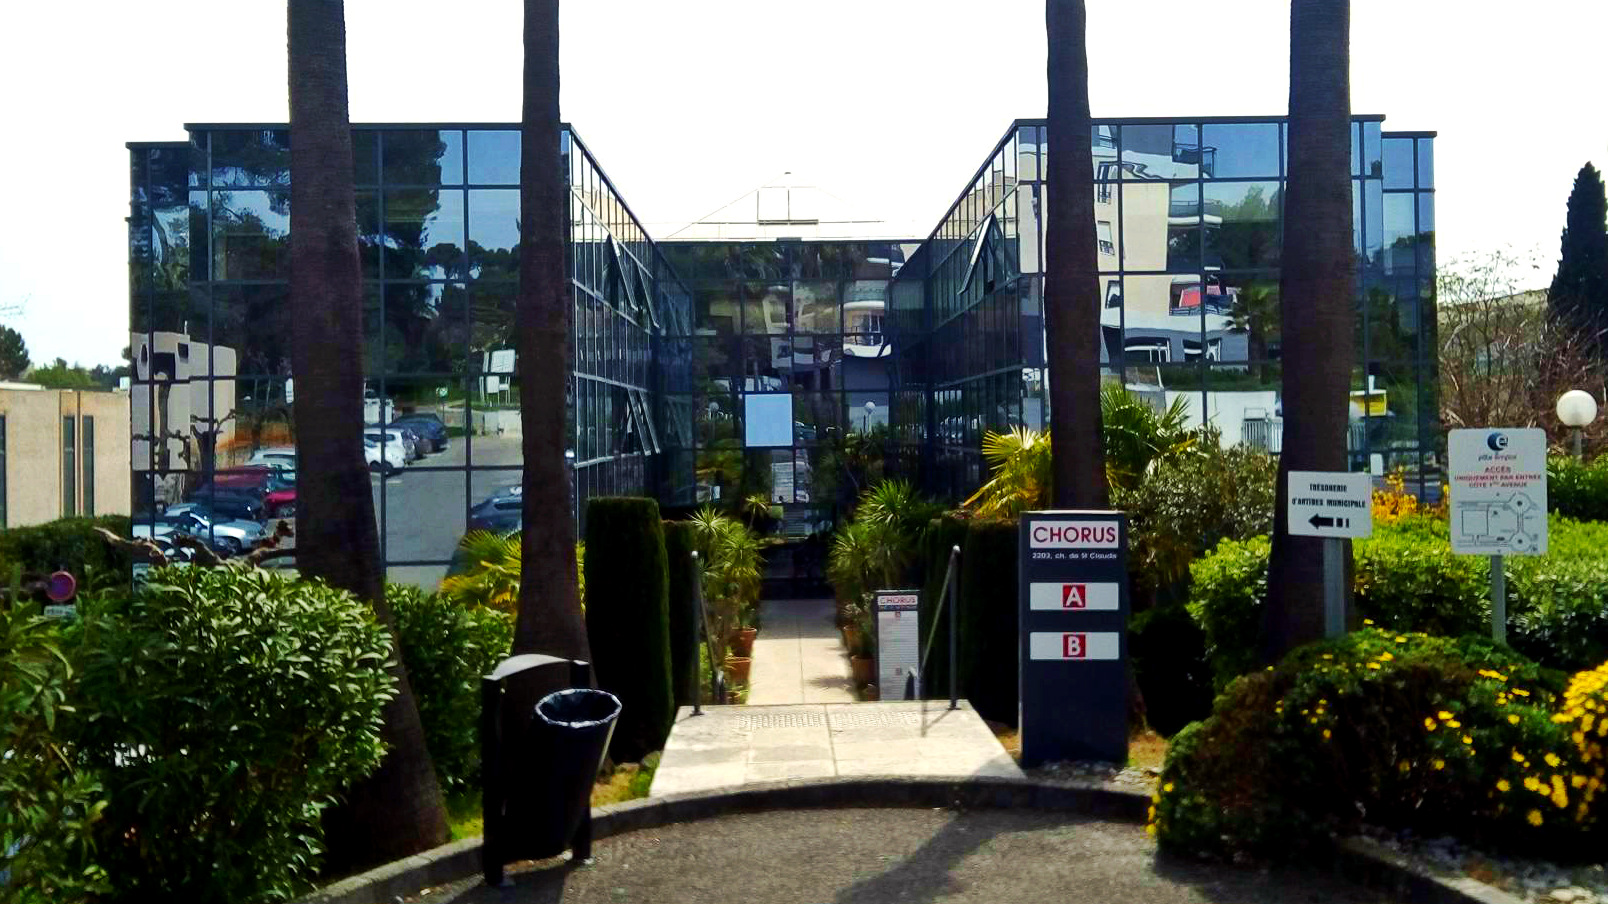
\includegraphics[width=9cm]{./img/supralog_building_3}
  \caption{\label{fig:mb_va_ast} Supralog}
\end{figure}


\paragraph{Les trois activités de l'entreprise\\}
Supralog est organisé en trois practices : Conseil / Technologie / Progiciel.\\
L'activité historique est l'édition de progiciels. Supralog développe deux gammes de solutions:
\begin{sitemize}
\item \textit{Topaze} qui permet la gestion des cabinets médicaux.
\item \textit{Intr@ssoc} qui est destiné à la gestion des grandes associations et fédérations.
\end{sitemize}

La deuxième activité de l'entreprise est le conseil, notamment pour \textit{Air France} et \textit{Amadeus}.\\
Enfin, il y a l'activité technologie qui porte sur la conception et le développement de systèmes d'information en architecture client-serveur. 

\paragraph{Quelques chiffres\\}
Les progiciels développés par SUPRALOG sont utilisés par plus de 40 000 personnes en France.\\
Les activités de technologie et de conseil regroupent plus de 15 clients.\\
L'entreprise a réalisé un chiffre d'affaires de plus de 7 millions d'euros en 2014 et présente une croissance de 114\% sur les 3 dernières années.

\subsection{Environnement de travail}
Mon stage se déroule au siège de l'entreprise au sein de l'équipe de développement du projet \textit{Topaze Web}.
L'équipe est constituée de 5 personnes: le chef de projet et directeur technique Nicolas Thibault, les ingénieurs développeurs Abdessalam Eljai et Anthony Biga, l'apprentis Tom Veniat et moi-même.

\subsection{Le projet Topaze Web et la gamme Topaze}
Topaze est une gamme de progiciels de gestion de cabinets pour professionnels des milieux
médicaux et paramédicaux. Cette gamme a été créée par Supralog en 1997 et est historiquement le
premier progiciel de santé à obtenir l'agrément SESAM Vitale, agrément permettant l’édition de
feuilles de soins électroniques.\\

Depuis 1997, Topaze a connu de nombreuses évolutions et a été publié et agréé en plusieurs versions ayant des architectures différentes. Lors de sa création Topaze était une application de bureau, puis il a évolué progressivement pour s'ouvrir à internet.
 
En 2015, le projet Topaze Web a été initié avec comme objectif de donner naissance à une application web multi tiers offrant les mêmes fonctionnalités que la version "Maestro" de Topaze.

%Ce projet, lancé en 2015, a pour objectif de permettre aux utilisateurs d’accéder au logiciel directement depuis leur
%navigateur web. Cette solution cloud possède différents avantages par rapport aux solutions classiques.
%Il n’est tout d’abord plus nécessaire d’installer un client lourd sur chaque poste utilisé par le
%professionnel de santé. Les risques de pertes de données ont été réduits ; cette architecture est déjà
%présente sur certaines versions de Topaze. En effet, les données étant stockées sur une machine
%distante, le dysfonctionnement de la machine d’un utilisateur n’impactera d’aucune manière ses
%données qui resteront accessibles depuis n’importe quel autre ordinateur se connectant à son compte.
%Au début de l’apprentissage, le projet Topaze Web avait déjà commencé depuis plusieurs
%mois. Il s’agit d’un projet utilisant majoritairement la spécification Java Enterprise Edition (J2EE) en
%combinaison avec les Frameworks Hibernate, Spring et JavaServer Faces (JSF).
%Les spécifications de l’application à réaliser sont basées sur l'existant : Topaze Web devra
%fournir des fonctionnalités similaires à celles de Topaze Maestro (version de Topaze initialement
%lancée en 2011). Tout en modernisant le design, l’interface utilisateur devra être suffisamment proche
%de celle de Topaze Maestro pour que les utilisateurs qui migreront prennent rapidement en main la
%nouvelle version. C’est dans ce cadre que cet apprentissage a débuté au sein de l’équipe de
%développement en charge de la réalisation de Topaze Web, composée d’un chef de projet et de deux
%autres développeurs.
%Le fonctionnement au sein de cette équipe suit les méthodologies agiles. Les fonctionnalités à
%développer en priorité sont choisies par le client, représenté par un membre de l’entreprise
%commercialisant Topaze. Le client suit étape par étape l’avancement du projet ce qui permet à l’équipe
%d’obtenir des retours réguliers.
%Ce rapport commencera par présenter plus précisément le projet, son contexte et ses objectifs
%avant d’exposer les problèmes posés au cours de cette première période d’apprentissage. Les attentes
%et le contexte dans lequel chaque mission s’inscrit y sont détaillés. La seconde partie exposera le
%travail réalisé, en expliquant plus précisément les méthodes employées pour remplir les missions qui
%ont été confiées. La démarche suivie ainsi que les résultats y sont décrits. La conclusion contient le
%bilan de cette première partie de l’année, ainsi que les compétences développées au cours de ces 2
%mois.

\subsection{Mission}
Mon rôle au sein de \textit{Topaze Web} est de me familiariser avec l'architecture du projet et ses technologies (J2EE, Hibernate, Spring et JSF) et de participer à la conception et au développement de l'application.\\

Les spécifications de l’application à réaliser sont basées sur l'existant : Topaze Web devra fournir des fonctionnalités similaires à celles de Topaze Maestro. Le design de l'application doit être modernisé, mais son ergonomie doit rester proche de l'existant pour ne pas déstabiliser l'utilisateur final. Enfin, un soin particulier doit être accordé à l'architecture, la conception et l'utilisation de patrons de conception lors du développement de l'application, afin de garantir la pérennité et la maintenabilité du logiciel au cours du temps. 

%Il s’agit d’un projet utilisant majoritairement la spécification Java Enterprise Edition (J2EE) en
%combinaison avec les Frameworks Hibernate, Spring et JavaServer Faces (JSF).
%Les spécifications de l’application à réaliser sont basées sur l'existant : Topaze Web devra
%fournir des fonctionnalités similaires à celles de Topaze Maestro (version de Topaze initialement
%lancée en 2011). Tout en modernisant le design, l’interface utilisateur devra être suffisamment proche
%de celle de Topaze Maestro pour que les utilisateurs qui migreront prennent rapidement en main la
%nouvelle version. C’est dans ce cadre que cet apprentissage a débuté au sein de l’équipe de
%développement en charge de la réalisation de Topaze Web, composée d’un chef de projet et de deux
%autres développeurs.

%TODO : Refactorer ou virer 
%\paragraph{Gestion de projet\\}
%La gestion du projet se fait en mode agile, selon une méthodologie proche du Scrum. 
%Les fonctionnalités à développer en premier son choisies par le client (la société IDEA d'IDLOG), puis les tâches sont chiffrées et réparties par le chef de projet. Le logiciel \textit{Jira} est utilisé pour l'assignation et le suivi des tâches. \\
%À la fin de chaque sprint, une réunion est organisé avec le client afin de montrer l'évolution du projet.


 % (2 pages)  done: 2

\newpage
\section{Problématique} % (5 pages) problématique de votre projet 
% (contexte du projet (workflow) + travail à réaliser + objectifs attendus)

\subsection{Contexte du projet}
Le développement du projet s'effectue en sprints, selon la méthode Scrum. Le contenu de chaque sprint est décidé d'un commun accord entre le chef de projet et le client. Le but est de réaliser en premier lieu les fonctionnalités les plus importantes fonctionnellement. 

\subsubsection{Mise en place du projet}
Durant cette première étape, il a fallu mettre en place l'architecture du projet, avec notamment les différents serveurs \textit{J2EE/Spring}, la base de données \textit{Postgre Sql}, l'\gls{ORM} Hibernate, la partie webapp avec \textit{JSF} et \textit{primefaces}.
Cette partie est abordée plus en détails, dans la section Architecture.

\subsubsection{Sprint 1}
Le sprint 1, qui a eu lieu avant mon arrivée, avait pour but la création des fonctionnalités de base permettant la gestion d'un cabinet.\\

La première fonctionnalité développée durant ce sprint permet la création d'un cabinet médical avec l'ajout de praticiens (kinésithérapeute, infirmiers etc.) et l'ajout de patients au cabinet.
La deuxième fonctionnalité porte sur la gestion des ordonnances pour les professions de type kinésithérapeute et infirmiers. Enfin, il y a la gestion des séances, avec la création d'un planning.


\subsubsection{Sprint 2}
Le second sprint du projet a commencé en début mars, peu de temps après mon arrivée. Il a été dimensionné pour tenir sur 6 semaines.
Les objectifs de ce sprint portent sur la création des fonctionnalités suivantes : 
\begin{itemize}
\item \textit{Les Feuilles de Soins Electroniques} : Il s'agit des feuilles de soins qui sont créées par le praticien et qui décrivent la prise en charge du bénéficiaire des soins ainsi que les différents actes réalisés et leur coût. La \gls{FSE} est mise à jour avec la carte vitale du patient à la réalisation du dernier acte et est ensuite transmise à l'assurance maladie.
\item \textit{Le contexte de facturation} : Il comprend la gestion des tarifications, des types de couverture et des types de prise en charge. Cette fonctionnalité nécessite la lecture des cartes SESAM Vitale.
\item \textit{Le dossier médical du patient} : Il contient une liste des documents associés au patient (ordonnances, factures, prescriptions, scans, images etc.)
\item \textit{Les cas métiers de la gestion des séances} : La gestion de base des séances faisait partie du sprint 1. Dans ce sprint ce sont les cas particuliers (i.e. les cas de figure issus du terrain) qui sont traités. Ces cas de figure couvrent par exemple l'annulation ou le décalage d'une séance par le praticien ou le client.
\item \textit{L'intégration continue et le TDD} : Ce n'est pas une fonctionnalité à proprement parlé, mais plus une amélioration des méthodes de production. L'intégration continue doit permettre une industrialisation de la production (tests lancés automatiquement lors du build et obtention de rapports portants sur la qualité du code). La méthodologie de TDD\footnote{TDD: Test-Driven Development (Développement dirigé par les tests).} porte sur la façon de développer et tester le logiciel. Elle doit permettre d'augmenter la qualité du code développé.
\end{itemize}

%TODO Compléter 
\subsubsection{Sprint 3} 
Ce troisième sprint prend place du 18 Avril au 23 Mai. 

%Les détails le concernant n'ont pour l'instant pas été abordés avec précision. Cependant, il est prévu que durant cette période, nous travaillions en collaboration avec des ergonomes et des designers afin d'améliorer l'expérience utilisateur.

Les objectifs de ce sprint portent sur la création des fonctionnalités suivantes :
\begin{itemize}
\item \textit{Ajout de placeholders dans un document RTF} : 
\item \textit{Gestion des modèles de documents RTF} : 
\end{itemize}

\subsubsection{Sprint 3}
Ce quatrième sprint prend place du 1er juin au 31 Août.
Les objectifs de ce sprint portent sur la création des fonctionnalités suivantes :
\begin{itemize}
\item \textit{Création d'un installer windows pour le driver Pyvital} :
\item \textit{Revue de l'authentification à l'API Sesame} :
\item \textit{Saisie d'un scan d'ordonnance} :
\end{itemize}

\subsection{Travail à réaliser}

La partie qui m'a été attribuée durant le sprint 2 est la mise en place du dossier médical du patient. Il s'agit d'une fonctionnalité du logiciel qui dépend des autres parties déjà développées (cabinets, praticiens, patients), mais qui est relativement indépendante. \\

Il s'agit d'une fonctionnalité présente dans \textit{Topaze Maestro}, qu'il faut créer dans \textit{Topaze Web}.
Une capture d'écran de la fonctionnalité du dossier médical de Topaze Maestro est visible en annexe \ref{fig:dossier_medical}.


\subsubsection{Les fonctionnalités du dossier médical dans Topaze Maestro}
\paragraph*{La liste des documents associés au patient\\}
La fonctionnalité principale est la liste des documents du patient. Cette liste contient différents types de documents : les ordonnances, factures, paiements, suivis, scans, courriers (textes), images, sons, objets \gls{OLE}. La liste peut être ordonnée selon le type de documents ou selon la date. Elle peut également être filtrée sur le type de documents.

\paragraph*{Le récapitulatif de chaque document\\}
Un panneau latéral permet à l'utilisateur d'avoir accès rapide aux informations du document qui est sélectionné dans la liste.

\paragraph*{La lecture ou la suppression de documents\\}
Chaque document de la liste doit pouvoir être ouvert ou supprimé.
L'ouverture d'un document est différente selon le type de celui-ci. Si c'est une ordonnance ou un document issu d'un regroupement d'information, l'ouverture provoquera l'affichage d'un nouvel écran. Si c'est une image, un pdf, ou un objet OLE, c'est un logiciel Windows qui s'ouvre. Enfin, si c'est un document \textit{richtext} (cas des courriers et prescriptions), un éditeur propre à Topaze permet l'édition. 

\paragraph*{Les modèles d'images\\}
Un onglet du menu latéral permet l'insertion d'une image à partir d'une librairie de modèles prédéfinis.

\paragraph*{Les documents textuels (\gls{RTF})\\}
L'utilisateur peut ajouter et éditer des documents textuels grâce à l'éditeur de texte intégré à Topaze. 
L'éditeur proposé est agrémenté de différentes fonctionnalités, telles que l'ajout d'images à partir d'une bibliothèque, l'utilisation de modèles de document et l'emploi d'emplacements paramétrés (placeholders).
Une capture d'écran de l'éditeur de texte de Topaze Maestro est disponible en annexe \ref{fig:editeur_texte}.

\subparagraph*{La bibliothèque d'images}
L'utilisateur peut insérer dans le document texte une image provenant de son ordinateur ou de la bibliothèque d'images.
La bibliothèque d'image présente plusieurs onglets thématiques et chaque onglet contient une liste d'images prédéfinies.

\subparagraph*{Les "placeholders"}
Les emplacements paramétrés (placeholders) sont des balises génériques qui peuvent être introduites dans un document texte et qui seront remplacées à la sauvegarde par leur valeur réelle (valeur en base de donnée).\\

Le mécanisme fonctionne en plusieurs temps : \\
D'abord, l'utilisateur sélectionne dans une arborescence l'information dont il a besoin (par exemple: la date d'une ordonnance) et le logiciel insère dans le texte la balise correspondante (dans notre cas : \textit{$[$ordonnance.numero$\_$securité$\_$sociale$]$}). \\
Ensuite, l'utilisateur remplit un contexte. Dans notre cas, le praticien aurait à choisir l'ordonnance ciblée.\\
Enfin, lorsque l'utilisateur clique sur "prévisualiser" ou "sauvegarder", l'emplacement est remplacé par sa valeur réelle.

\subparagraph*{Les modèles de texte}
Les modèles de texte sont des document RTF contenant des placeholders, qui ont vocation à être réutilisés.\\
Ces modèles sont accessibles via une bibliothèque similaire à celle des images. 
Lorsque l'utilisateur ouvre un modèle, il peut le modifier et l'enregistrer comme un document normal. 

\paragraph*{L'ajout de scans \\}
L'utilisateur a la possibilité de numériser un document dirèctement en cliquant sur un bouton du menu latéral. Il peut également insérer un document déja scanné, via le même bouton.

\paragraph*{L'ajout d'objets OLE\\}
Le protocole OLE (Object Linking and Embedding) est un protocole mis au point par microsoft permettant la liaison et l'incorporation d'objets. Cela permet à différents logiciels de se transmettre des objets. \\
Dans topaze, l'utilisateur peut donc insérer tout objet/document qui implémente l'interface \textit{IOleObject}. Concrètement, il peut donc insérer un document word, une image paint, une vidéo etc. et lorsqu'il cliquera sur "voir", le logiciel approprié de windows s'ouvrira pour lui permettre de visualiser et/ou éditer le document.
Cette fonctionnalité est trés puissante car elle permet le support d'un trés grand nombre de documents. 

\paragraph*{L'enregistrement de sons\\}
L'utilisateur peut enregistrer un son en cliquant sur un bouton du menu. Cela lui ouvre un logiciel d'enregistrement de sons de Windows.
 
%TODO refaire de façon plus globale
\subsection{Les objectifs précis attendus}
Les objectifs attendus lors du sprint 2 : 
\begin{itemize}
\item L'accès au dossier médical du patient.
\item L'édition de documents texte (sans modèle).
\item L'ajout de documents numériques au dossier d'un patient.
\end{itemize}

Pour chaque objectif, les tâches suivantes sont à réaliser :
\begin{itemize}
\item Analyse de l'existant (fonctionnalités et comportements de Topaze Maestro) 
\item Etude de la faisabilité des différentes fonctionnalités.
\item Discussion du besoin avec le chef de projet et/ou la maîtrise d'ouvrage.
\item Proposition d'une solution qui réponde fonctionnellement au besoin.
\item Spécification  du modèle métier (entités de la base de données) qui réponde au besoin.
\item Spécification de l'API Rest.
\item Spécification des interfaces graphiques si besoin.
\item Implémentation de la solution (backend + frontend) dans Topaze Web.
\end{itemize}

\subsection{Les enjeux pour l'entreprise}
%TODO % (5 pages)  done: 3.2

\newpage
\section{Solutions techniques} % (10 pages) Solutions techniques mises en oeuvre

%synthèse de l'existant (couverture fonctionnelle existante (architecture logicielle par ex.), contraintes inhérentes au projet (outils, librairies, …), s'appuyant sur une bibliographie précise

%description de la (ou des) solution(s) envisagée(s) et des outils qui seront utilisés

%protocole d'évaluation envisagé pour valider votre solution ou mesurer son efficacité

\subsection{Synthèse de l'existant} % (objectif perso : 4 pages)
\subsubsection{Architecture logicielle}
\paragraph*{Architecture 3-tiers\\}
Topaze web est bâti selon une architecture 3-tiers : 
\begin{sitemize}
\item la \textit{couche présentation} qui sert à l'affichage des informations et qui tourne sur le navigateur du client.
\item la \textit{couche métier} qui contient la logique applicative.
\item la \textit{couche d'accés aux données} qui garantie la persistance des données (base(s) de données). 
\end{sitemize}

\paragraph*{Les utilisateurs\\}
Le projet Topaze Web aura deux types d'utilisateurs : 
\begin{sitemize}
\item \textit{Les infirmiers, kinésithérapeutes et autres professionnels de la santé} qui utiliseront Topaze au quotidien pour la gestion des feuilles de soins, de la facturation, des dossiers patients etc. 
\item \textit{Le service technique d'IDEA} (la société soeur de Supralog qui commercialise Topaze) : qu’il s’agisse des personnes
chargées d’administrer les comptes utilisateurs et cabinets ou les personnes étant au SAV, ils
utiliseront l’application pour gérer les abonnements et répondre aux problèmes techniques des
clients finaux.
\end{sitemize}

Pour résumer, voici une schéma de l'architecture 3-tiers de Topaze Web :
\begin{figure}[H]
  \centering
  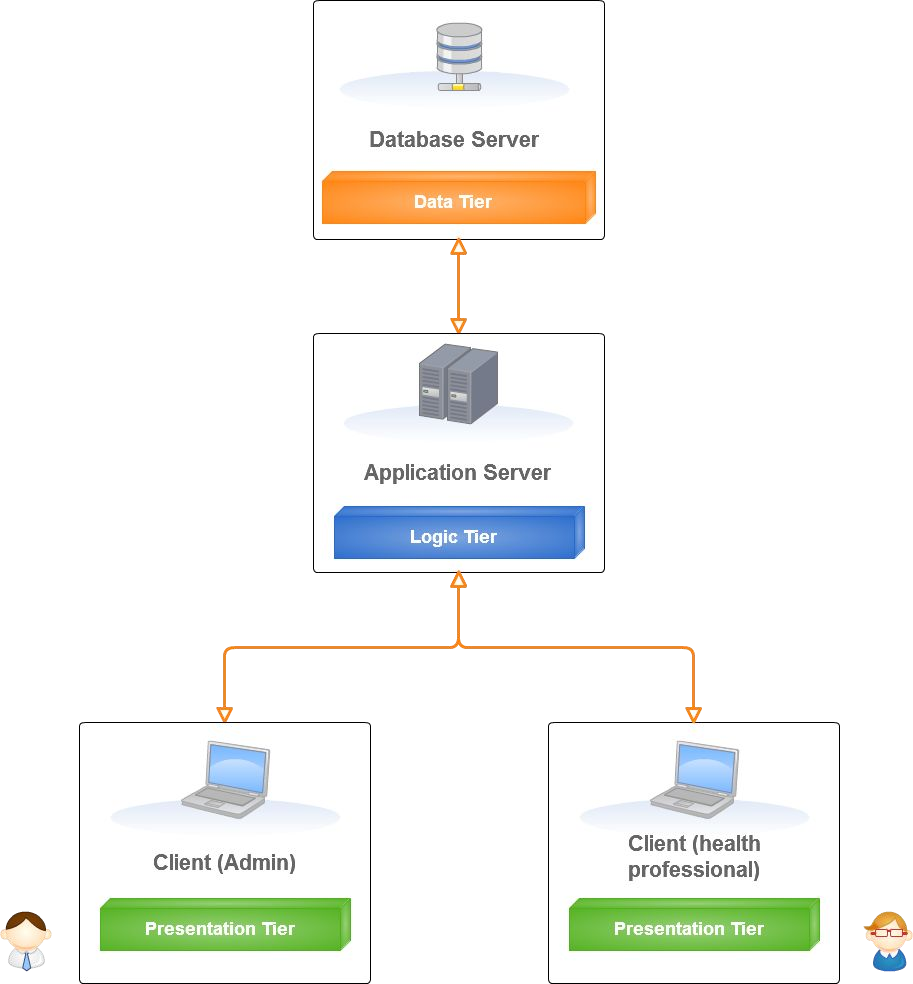
\includegraphics[width=8cm]{./img/architecture1}
  \caption{\label{fig:mb_va_ast} Schéma de l'architecture 3-tiers (créé par Tom Veniat, utilisé avec son accord)}
\end{figure}

Afin de satisfaire les besoins de ces deux types d'utilisateurs, deux applications qui accèdent aux mêmes données ont été crées: 

\begin{sitemize}
\item \textit{Topaze} : l'application utilisée par les professionnels de la santé. 
\item \textit{Opale} : l'application utilisée par les administrateurs.
\end{sitemize}

\paragraph*{L'application Topaze\\}
L'application Topaze a été scindée en deux parties : \textit{Topaze REST} et \textit{Topaze Webapp}.\\
\textit{Topaze Rest} est un serveur REST, à accès sécurisé par token. Il réalise les opérations liées à la logique métier et il fait persister les données en base.\\
Topaze Webapp gère la mise en forme des données avant affichage. Son accès est sécurisé via une authentification par sessions. Elle contacte topaze REST afin de rapatrier les données, puis elle les met en forme avant de les envoyer au client (le navigateur).

\paragraph*{L'application Opale\\}
Opale et Topaze ont une base de données en commun. De cette manière, un administrateur d'Opale peut ajouter un utilisateur qui sera ensuite utilisable dans Topaze. \\
Les deux applications sont séparées car elles sont utilisées par des utilisateurs différents, mais également parce qu'elles effectuent des tâches de nature différente. En effet, les tâches réalisées par les administrateurs, dans Opale, se résument à des opérations CRUD \footnote{CRUD: Create, Read, Update, Delete} sur la base de données. Dans Opale, il n'y a donc pas ou peu de logique métier. 
De ce fait, le code de l'application Opale est presque entièrement générée au moyen du \textit{Skeleton Generator}.\\ \\
Le \textit{Skeleton Generator} est un projet open-source, développé par le chef de projet, qui permet de faire du M2C \footnote{M2C: Modèle To Code}. Dans opale, on décrit donc les modèles de données via un fichier XML (cf annexe \ref{fig:xml}), puis le générateur est utilisé pour créer les entités en base de données, générer le code des DAO \footnote{DAO: Data Access Object} qui serviront pour Opale et Topaze et générer tout le code d'Opale (les composants-métier, les objets métiers, les services, l'api rest, ainsi que l'application web). 

\paragraph*{L'application Sesame\\}

La manipulation des Feuilles de Soins Electroniques (FSE) et la facturation nécessitent la lecture d'informations présentes sur la carte vitale du patient. D'autre part, les logiciels utilisant les FSE sont soumis à l’obtention d’un agrément délivré
par les représentants des organismes d’Assurance Maladie. Cet agrément est obtenu après de
nombreux tests vérifiant que le logiciel en question respecte un cahier des charges très précis.\\
La gestion de la facturation et des FSE étant nécessaire à l’application, mais pouvant
être externalisée, c’est une troisième application qui en a la responsabilité. \\
Cette troisième application nommée \textit{Sesame} répond à trois problématiques : 
\begin{sitemize}
\item La communication avec le lecteur de cartes vitales.
\item La facturation des actes réalisés par les praticiens, en fonction des informations du patient présentes sur la carte vitale.
\item La communication avec Topaze et la restriction des accés à la carte vitale.
\end{sitemize}

Afin de pouvoir communiquer avec la carte vitale un driver doit être installé sur la machine de l'utilisateur. Par la suite, le serveur Sesame communique avec le driver via des websockets afin d'avoir accès aux informations de la carte vitale.

\paragraph*{Schéma d'architecture global\\}
Voici le schéma d'architecture globale représentant l'architecture 3-Tiers et la communication entre les différentes applications :
\begin{figure}[H]
  \centering
  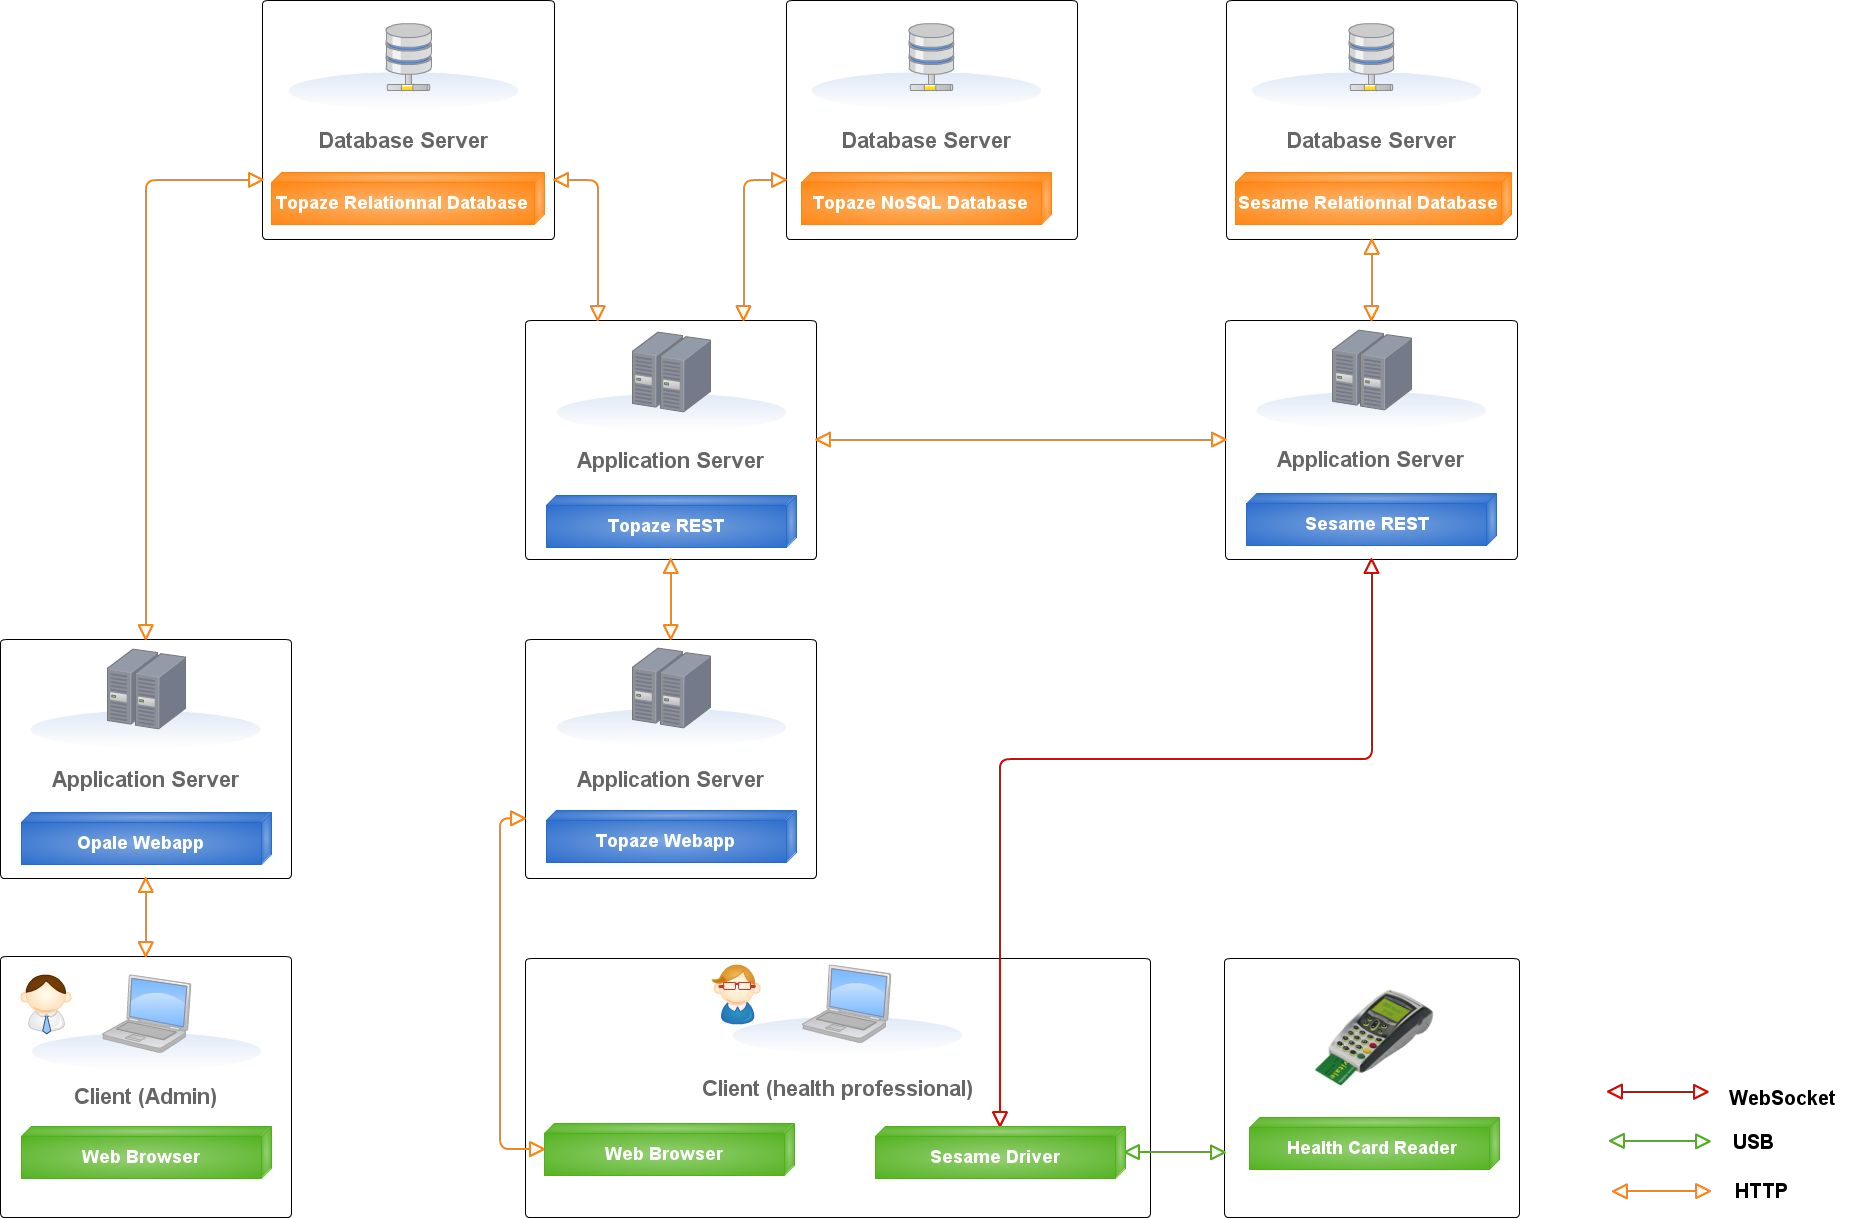
\includegraphics[width=18cm]{./img/architecture2}
  \caption{\label{fig:mb_va_ast} Schéma d'architecture global (créé par Tom Veniat, utilisé avec son accord)}
\end{figure}

\subsubsection{Technologies utilisées}
Les technologies utilisées par le projet sont :
\begin{sitemize}
\item Bases de données : PostgreSQL pour les modèles de données, MongoDB et GridFS pour les fichiers.
\item ORM : Hibernate
\item Serveur : Tomcat
\item Backend : Java et Spring
\item Front-End : JSF et Primefaces
\end{sitemize} 

\subsection{Solution envisagée}
\subsubsection{Conception et implémentation du dossier médical}

%\item Analyse de l'existant (fonctionnalités et comportements de Topaze Maestro) 
%\item Etude de la faisabilité des différentes fonctionnalités.
%\item Discussion du besoin avec le chef de projet et/ou la maitrise d'ouvrage.
%\item Proposition d'une solution qui réponde fonctionnellement au besoin.
%\item Spécification  du model métier (entités de la base de données) qui réponde au besoin.
%\item Spécification de l'API Rest.
%\item Spécification des interfaces graphiques si besoin.
%\item Implémentation de la solution (backend + frontend) dans Topaze Web.
\paragraph{Analyse de l'existant\\}
Le dossier médical de Topaze Web doit, si possible, apporter les mêmes fonctionnalités que celui présent dans Topaze Maestro.
La première étape de conception a donc consisté à faire une analyse de l’existant et à lister les fonctionnalités présentes (il s’agit de la liste décrite dans la section Problématique).

\paragraph{Etude de la faisabilité\\}
Ensuite, j'ai étudié la faisabilité des différentes fonctionnalités et les ai triées en fonction de leur difficulté à être implémentées en web. La plupart des fonctionnalités peuvent être créées sans difficulté, cependant certaines ont soulevé des questions :

\subparagraph*{Le cas des objets OLE} est particulier, car il s'agit là d'un protocole de Microsoft à destination de Windows. 
Il ne peut donc pas être utilisé dans une solution web. À ce niveau, il était donc nécessaire de savoir quels types d'objets devaient être supportés et si la fonctionnalité était vraiment importante. En effet, chaque objet à supporter nécessite de batir une solution sur mesure.\\
Après discussion avec le chef de projet, il a été décidé que l'utilisation des objets OLE ne serait pas géré à proprement parlé dans l'application. Cependant, l'utilisateur peut, s'il le désire, télécharger différents types de fichiers sur l'application et les récupérer ensuite pour les éditer avec ses propres logiciels.

\subparagraph*{Le cas des documents RichText} a lui aussi demandé un traitement spécifique. Dans Topaze Maestro, les documents au format richtext peuvent être téléchargés puis édités directement depuis l'application. En web, l'édition de documents au format richtext n'est pas habituelle. En revanche, de nombreux éditeurs \gls{WYSIWYG} existent et permettent d'éditer du Markdown, du BBCode ou du HTML. J'ai donc choisi d'intégrer un composant extérieur afin de remplir cette tâche. Afin que les utilisateurs de Topaze Maestro puissent réutiliser leurs données dans Topaze Web, il a été décidé que les fichiers au format RTF seraient transformés en HTML au moyen d'un traitement batch en cas de migration de donnée. \\
Les choix techniques et l'intégration du composant seront décrits dans la section \ref{editeur_section}.

\subparagraph*{Le cas des sons} est particulier. Pendant longtemps, cette fonctionnalité a été implémentée en web en utilisant du flash. Aujourd'hui, la balise audio d'HTML5 permet de lire des sons de façon native dans les navigateurs. Cette fonctionnalité d'HTML5 est supporté par quasiment tous les navigateurs, sauf IE8 \footnote{Support de la balise audio : http://caniuse.com/\#feat=audio}. \\
En ce qui concerne l'enregistrement des sons (possible dans Topaze Maestro via un objet OLE), HTML5 offre l'API getUserMedia qui permet d'accéder au flux audio ou vidéo d'un périphérique externe. Cependant, le support de cette fonctionnalité n'est pas encore assuré par tous les navigateurs \footnote{Support de l'API getUserMedia : http://caniuse.com/\#feat=stream}. Afin de résoudre la question du support des navigateurs, des bibliothèques open-source telles que \textit{getUserMedia.js}\footnote{getUserMedia.js : https://github.com/addyosmani/getUserMedia.js} ont été développées. Ces bibliothèques utilisent la getUserMedia API si elle est disponible et utilisent Flash si ce n'est pas le cas.

\paragraph{Elaboration d'une solution\\}
Afin d'élaborer une solution, j'ai commencé par réaliser un diagramme de classe d'analyse modélisant les différents objets qui interviennent dans le dossier médical:

\begin{figure}[H]
  \centering
  \includegraphics[width=11cm]{./img/class}
  \caption{\label{fig:mb_va_ast} Diagramme de classe d'analyse du dossier médical.}
\end{figure}

Dans ce diagramme d'analyse, on peut voir que le dossier médical est constitué de deux types de documents : ceux que j'ai appelé les "Documents MIME" qui correspondent à des fichiers binaires (sons, images, textes) et les autres, qui sont des objets métiers manipulés dans l'application.\\

Une fois ce diagramme réalisé s'est posée la question de la persistance des données. Avant toute chose, j'ai regardé le contenu de la base de données afin de savoir quelles entités étaient déjà présentes.\\
Voici le modèle conceptuel de la base de données au départ (seules les entités concernant le cas étudié ont été représentées)  :

\begin{figure}[H]
  \centering
  \includegraphics[width=15cm]{./img/existing_model}
  \caption{\label{fig:mb_va_ast} Modèle UML conceptuel de la base de donnée, au départ.}
\end{figure}

Dans la base de donnée, les prescriptions étaient déja présentes. Il restait donc à ajouter les documents issus de fichiers. \\
Voici donc l'ajout que j'ai réalisé au modèle de donnée : 
\begin{figure}[H]
  \centering
  \includegraphics[width=13cm]{./img/created_model}
  \caption{\label{fig:mb_va_ast} Modèle UML illustrant les ajouts à la base de données.}
\end{figure}

Ensuite, s'est posée la question du stockage du contenu des fichiers. Deux choix étaient possibles : les stocker en base, ou directement dans un système de fichier. Cette question s'était déjà présentée plus tôt dans le projet, et l'équipe avait décidé de stocker les données binaires dans une base de données Mongo DB munie de GridFS. Ce choix a été fait pour les caractéristiques de disponibilité et de scalabilité propre à MongoDB.\\
La base de données PostgreSQL est donc utilisée pour stocker les méta données liées au fichier et leur contenu est stocké dans MongoDB. Lorsqu'on a besoin du contenu d'un fichier, on récupère son id dans Postgre et l'on fait une requête dans MongoDB pour obtenir son contenu. La convention choisie est que le filename dans Mongo correspond à l'id du document dans Postgre. \\

Dans MongoDB, deux collections sont utilisées, par défaut, par GridFS pour stocker les fichiers :  
\begin{figure}[H]
  \centering
  \includegraphics[width=12cm]{./img/gridfs}
  \caption{\label{fig:mb_va_ast} Collections utilisées par GridFS pour le stockage des fichiers.}
\end{figure}
La collection \textit{Chuncks} sert à stocker les données du fichier et la collection \textit{Files} sert à stocker les méta-données du fichier.

\paragraph{Phase d'implémentation\\}
Une fois le modèle de données mis en place, il ne reste plus qu'à réaliser l'implémentation dans Topaze Rest et \textit{Topaze Webapp}. 
À ce niveau, différentes classes sont à implémenter dans la \textit{Topaze Webapp} et dans \textit{Topaze Rest}. Afin de comprendre quelles classes sont à implémenter, voici un schéma illustrant la requête permettant d'obtenir le dossier médical (le diagramme est également fourni en plus grand, en annexe \ref{fig:diag_seq}, pour les lecteurs sur papier):
\begin{figure}[H]
  \centering
  \includegraphics[width=17cm]{./img/diag_seq}
  \caption{\label{fig:mb_va_ast} Diagramme de séquence modélisant la requête du dossier médical.}
\end{figure}

Comme on peut le voir, l'architecture de la \textit{webapp} suit un modèle MVC. Du côté de \textit{Topaze Rest}, il y a plusieurs packages : 
\begin{itemize} 
\item \textit{API} qui définit les services et les modèles (qui correspondent à des vues simplifiés des objets tirés de la base)
\item \textit{REST} qui définit les les contrôleurs (qui font le mapping entre une url et un service)
\item \textit{REST Client} qui définit des services clients utilisés par la web-app pour contacter les contrôleurs.
\item \textit{Business components} qui définit les objets tels que les mappers qui permettent de créer des vues ad-hocs à partir des modèles issus de la base de données.
\end{itemize}

Enfin, on utilise également les DAO \footnote{DAO: Data Access Object} définis dans Opale qui permettent d'obtenir les informations de la base de données.\\

Une capture d'écran du dossier médical de Topaze Web est disponible en annexe \ref{fig:dossier_web}.

\subsubsection{Choix et intégration de l'éditeur de texte}\label{editeur_section}
% Choix editeur + licence permissive et non contaminante
% Problème Richtext et données existantes

L’édition de texte est une fonctionnalité importante de Topaze Maestro. Il fallait donc qu’un éditeur soit implémenté ou intégré. De nombreux éditeurs de texte de qualité ont déjà étés développés et il en existe sous toutes les licences. Il a donc été choisi d’intégrer un composant existant. Cela permet d’avoir un composant robuste, bien documenté, éprouvé par toute une communauté et en continuelle évolution.\\

Les critères que j’ai pris en compte lors du choix étaient la notoriété du projet, le nombre de contributeurs et d’utilisateurs, son ancienneté, le support proposé, le nombre de fonctionnalités offertes, les possibilités de configuration, la possibilité de greffer de nouveaux plugins et enfin, la licence.\\

La licence était une question importante car Topaze Web est destiné à être commercialisé. Il n’était donc pas possible de choisir un éditeur distribué sous une licence à fort copyleft (par exemple la GPL). Un tel choix aurait contraint Topaze Web à être lui-même distribué sous licence GPL.\\

Pour finir, l’éditeur CKEditor a été choisi car il propose une licence LGPL, dispose d’une bonne communauté, de nombreux plugins et de la possibilité d’ajouter facilement ses propres plugins.

\subparagraph*{Intégration de l’éditeur\\}
L’intégration se fait très facilement en ajoutant la librairie de l’éditeur. Il ne reste plus ensuite qu’à gérer le flot de données qui circulent entre l’éditeur et l’application. Du javascript est utilisé pour gérer la sauvegarde lors du click sur le bouton ou périodiquement si l’utilisateur ne sauvegarde pas.\\

Par la suite d’autres modifications seront apportées (vue réaliste faisant apparaître les pages telles qu’elles seront imprimées, galerie d’image, import d’images).\\

Une capture d'écran de l'éditeur de texte de Topaze Web est disponible en annexe \ref{fig:editeur_web}.

\subsubsection{La bibliothèque d'images}
Dans Topaze Maestro, la bibliothèque d'images contient uniquement des images prédéfinies. Dans la version web, il a été décidé qu'elle puisse également contenir des images importées par l'utilisateur.\\
De manière à ce que la bibliothèque soit simple à gérer, nous avons décidé (le chef de projet et moi) de créer un gestionnaire de fichiers avec une arborescence de dossiers.\\

\paragraph*{Elaboration du modèle de données\\}
Lors de la conception du modèle, la contrainte suivante devait être prise en compte : \\
Lorsqu'un utilisateur supprime une image de sa bibliothèque, si celle-ci a été insérée dans un document, elle doit continuer d'y appraître. \\
Ainsi, il était nécessaire de séparer en base, l'apparition d'une image dans la bibliothèque de son stockage pour utilisation dans les documents texte. \\
J'ai donc créé le modèle suivant : 

%TODO : MCD des directory, userImageAddress, UserImage : vérifier si on met les ID ou pas ...
\begin{figure}[H]
  \centering
  \includegraphics[width=12cm]{./img/directory_entities_concept}
  \caption{\label{fig:mb_va_ast} Modèle UML conceptuel du système de gestion de fichiers.}
\end{figure}

\paragraph*{Spécification de l'API REST\\}
En ce qui concerne l'API REST, elle contient les opérations de CRUD\footnote{CRUD: Create Read Update Delete} sur les dossiers et leur contenu.
L'API expose donc les urls suivantes concernant les dossiers : 
%TODO : à vérifier.
\begin{itemize}
\item GET /account/models/directory/{directoryId}
\item DELETE /account/models/directory/{directoryId}
\item POST /account/models/directory
\end{itemize}

Concernant les images contenues, ont trouve :
\begin{itemize}
\item GET /account/models/directory/{directoryId}/picutre/{pictureId}/content
\item DELETE /account/models/directory/{directoryId}/picutre/{pictureId}
\item POST /account/models/directory/picutre
\end{itemize}

\paragraph*{Modèle de l'API\\}
L'API REST récupère les donneés de la base au moyen de DAOs\footnote{DAO: Data Access Object} et peuple des objets métiers qu'elle va ensuite retourner.\\

Pour la base de donnée, il était plus simple de stocker l'arborescence de façon ascendante (chaque fichier contient l'id du dossier parent). Mais, concernant les objets métiers (qui eux seront exposés), on souhaite que l'arborescence soit stockée de façon descendante, pour que leur usage soit naturel.
En effet, les objets métiers sont ensuite utilisés pour générer les vues en HTML. Dans ce cas, on a donc en général accés à un dossier et on souhaite obtenir la liste de ses fils. \\

Pour représenter ce type de modèle, on pense naturellement au design pattern composite : \\
\begin{figure}[H]
  \centering
  \includegraphics[width=12cm]{./img/directory_entities_concept}
  \caption{\label{fig:mb_va_ast} Modèle UML de classes du système de fichiers, suivant le patron de conception composite.}
\end{figure}

Cependant, les objets retournés par l'API REST seront transmis par le réseau et devront donc être sérialisés. Hors, l'outil utilisé pour la sérialisation (Jackson), ne gère pas nativement le polymorphisme de java. \\
Le moyen utilisé pour pouvoir le faire quand même consiste à utiliser des annotations Jacksons, ou à inclure un champ "type" dans le json retourné par l'API. Cependant, ce choix est couteux car il impose des contraintes fortes sur le client utilisant l'API: l'usage de Jackson ou l'ajout d'un mécanisme particulier pour parser les objets reçus.\\

N'ayant que deux types d'objets, j'ai donc préféré briser l'héritage.

%TODO  OK: schéma du nouveau modèle. => NON c'est hiddeux ...

\paragraph*{Implémentation de la partie WebApp\\}
La webapp effectue des traitements assez standards. Elle effectue des appels aux services REST pour obtenir les dossiers et leur contenu et expose un certain nombre de méthodes utilisables par les vues JSF grâce un controlleur.
Le modèle utilisé par la webapp est rudimentaire car il ne fait qu'encapsuler les objets métiers obtenus de l'API REST et stocke en plus quelques variables d'états pour la vue.

\paragraph*{Spécification de l'interface graphique\\}
Avant d'implémenter la vue en JSF dans l'application, j'ai réalisé un prototype en HTML et javascript dans plunker.
Plunker est un éditeur en ligne pour le front-end. Il permet de faciliter la programmation fron-end en proposant un aperçu en temps réel, une inclusion de librairie simple, une gestion de version, un stockage privé du code et un partage simple et rapide du résultat avec un tiers.

Une fois que le résultat était satisfaisant, il a suffit de convertir une partie du HTML en JSF pour l'intégrer au code.

\paragraph*{Création d'un composant réutilisable\\}
Le gestionnaire de fichier utilisé pour la bibliothèque d'image a vocation à pouvoir être réutilisé à d'autres fin.
J'ai donc créé un composant réutilisable.

En JSF, plusieurs choix sont possibles pour créer des composants réutilisables : 
\begin{itemize}
\item Les \textit{Inclusions de code} : c'est la solution la plus rudimentaire. Elle consiste à extraire un morceau de code et à l'inclure ensuite en utilisant des \textit{<ui:include>} et \textit{<ui:param>}. Cette solution est adoptée lorsque le code inclus n'est pas ou peu paramétrable et n'a pas une sémantique trés forte (i.e. le code ne représente pas réellement un composant à lui seul).
\item Les \textit{Custom Tags} : il s'agit de la solution la plus légère lorsqu'on souhaite créer un composant réutilisable. C'est une méthode trés proche des inclusions de code, mais qui offre une interface plus propre. Elle permet une librairie de nouvelles balises jsf, qui peuvent accepter des paramètres en attributs. \\
Il s'agit de la solution choisie lorsqu'on souhaite éviter une répétition de code et que ce dernier remplit une fonction précise (notion de composant).
\item Les \textit{Composite Components} : cette solution est trés semblable aux tags, mais elle est plus coûteuse en temps de traitement. Elle a l'intérêt de présenter un passage de paramêtres plus propre que les tags et de nécessiter moins de code.\\
Cette solution est en générale choisie, lorsqu'on souhaite agréger plusieurs composants ou tags pour en créer un nouveau qui a son propre comportement.
\item Les \textit{Custom Components} : ce sont des composants définis en java (et non plus en JSF). Pour en créer, il faut définir une classe qui assurera le rendering du composant.\\
Cette solution est beaucoup plus lourde que les autres en temps de développement et en quantité de code. Elle est utilisée lorsque les solutions précédentes ne sont pas suffisantes. On l'utilise par exemple, pour ajouter un nouveau comportement à un composant existant, utiliser des évènements java ou avoir un rendu HTML particulier. 
\end{itemize}

Pour le gestionnaire de fichiers, mon choix s'est porté sur les tags, car la solution est performante et s'avère suffisante pour traiter le besoin.\\
Le code remplit une fonctionnalité précise et homogène (notion de composant), donc une inclusion de code n'était pas suffisante. Le code n'aggrège pas d'autres composants, donc il n'y avait pas nécessité d'utiliser un \textit{composite component}. Enfin, l'usage d'un \textit{custom component} aurait été disproportionné car coûteux et inutile (absence de nécessité du rendering en Java).\\

\subsubsection{Les "placeholders"}
Dans l'éditeur de texte de Topaze Maestro, une fonctionnalité permet d'utiliser des emplacements paramétrés (placeholders) qui sont remplacés à la sauvegarde par leur valeur réelle (en base de donnée). \\
Cette fonctionnalité est trés puissante car elle permet à l'utilisateur d'inclure dans ses documents des sortes de pointeurs vers des données présentes en base. \\

\paragraph*{Faisabilité\\}
La faisabilité de la foncionnalité reposait sur trois éléments : %TODO expliciter plus ?
\begin{itemize}
\item La possiblité d'insérer des balises html complexes dans ckeditor.
\item La possibilité de créer un lien entre une balise du texte et une donnée en base.
\item La possibilité de remplacer la balise par sa valeur.
\end{itemize}

\paragraph*{La solution mise en place}
\subparagraph*{L'insertion de placeholders dans l'éditeur}
Le premier pas pour réaliser la fonctionnalité était d'ajouter un plugin à l'éditeur pour insérer les placeholders.\\
Dans l'éditeur, les placeholders doivent avoir un formattage spécifique pour être reconnaissables, ne pas pouvoir être éditables et le html doit éventuellement pouvoir encapsuler des données (attributs \textit{data-*} de HTML).\\

Le plugin a été réalisé de la même manière que pour la bibliothèque d'image : en ajoutant un fichier \textit{plugin.js} et en utilisant une modale bootstrap.\\
En ce qui concerne les balises : le CSS permet de leur donner l'allure souhaitée, l'API de CKEditor permet d'insérer du HTML dans le texte à l'endroit du curseur et la liste blanche des éléments acceptés par l'éditeur est modifiable via un fichier de configuration.

\subparagraph*{Le lien entre les données vues par l'utilisateur et les données en base}

Lorsque l'utilisateur souhaite insérer un placeholder, il doit d'abord le sélectionner dans une arborescence. 
Lors du click sur une feuille de l'arborescence, le placeholder est inséré.  \\

Lors de la manipulation, l'utilisateur voit donc deux types d'informations : 
\begin{itemize}
\item les noeuds de l'arborescence.
\item les placeholders.
\end{itemize}

Pour pouvoir construire l'arborescence et effectuer le remplacement des placeholders par leur valeur, les informations visibles par l'utilisateur doivent être reliées à des objets métiers de l'API.
Dans ce but, deux solutions étaient disponibles : 
\begin{itemize}
\item utiliser des tables en base de données.
\item socker l'information dans les classes java. % annotations spring + introspection java
\end{itemize}

En JSF, on est déjà capable d'insérer dans les vues des informations provenant du modèle grâce aux EL \footnote{EL: Expression Language}. Par exemple, l'expression \textit{\#$\{$prescriptionView.date$\}$} sera remplacée par sa valeur par JSF, lors de la génération du HTML. Lors du remplacement d'un placeholder par sa valeur, on doit donc faire le lien entre cette notation pointée et le nom du placeholder.\\

\textbf{La première approche} conciste à ré-utiliser la table directory \footnote{la table directory est celle introduite pour gérer l'arborescence du gestionnaire de fichier} pour les dossiers de l'arborescence et à ajouter une nouvelle table pour les feuilles. Cette deuxième table sert à faire le lien entre les noms des placeholders, la notation pointée de java et le libellé à utiliser dans l'arborescence:\\

\begin{figure}[H]
  \centering
  \includegraphics[width=12cm]{./img/placeholders}
  \caption{\label{fig:mb_va_ast} Modèle UML conceptuel de base de données pour l'arorescence des placeholders.}
\end{figure}


\textbf{La deuxième approche} vise à utiliser les capacités de Java pour stocker l'information nécessaire directement dans le code.\\
Pour créer l'arborescence, il est possible d'utiliser la fonctionnalité d'introspection de java. L'introspection permet de prendre une classe et de parcourir ses propriétés et méthodes. Avec cette technique, on peut parcourir les objets métiers à exposer par les placeholders pour remplir un arbre (qui sera utilisé pour construire l'arborescence dans la vue). \\
Pour faire le lien entre les propriétés des objets métiers, les libellés de l'arbre et le nom des placeholders, on ajoute des annotations sur les propriétés des classes.\\
Par exemple :

\begin{figure}[H]
  \centering
  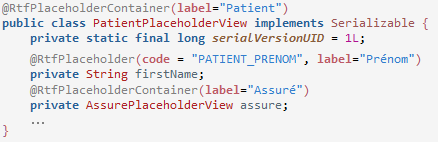
\includegraphics[width=11cm]{./img/annotations1}
  \caption{\label{fig:annotations} La classe PatientAnnotationView a été annotée avec 2 annotations (RtfPlaceholderContainer et RtfPlaceholder) afin de pouvoir être ensuite introspectée et servir à créer l'arborescence de placeholders.}
\end{figure}

\textbf{Pour comparer les deux solutions :} en terme de co\^ut, la première approche bénéficie d'un accés direct à l'information, mais celle-ci requiert un accés à la base de données et la reconstruction de l'arbre. Dans la deuxième approche, l'accés à l'information n'est pas direct, il faut parcourir les classes (couteux) et également reconstruire l'arborescence, mais on évite un accés à la base de données.\\
En ce qui concerne la maintenabilité, la deuxième solution est meilleure, surtout pour le lien entre le placeholder et la notation pointée.\\
Finalement, c'est donc la deuxième solution qui a été retenue et que j'ai implémentée.


\subparagraph*{Le remplacement des placeholders par leur valeur}
Le remplacement des placeholders par leur valeur a lieu lors de la sauvegarde du document, ou lorsque l'utilisateur demande une prévisualisation.\\

Trouver des expressions tokenisées dans un texte et les remplacer par leur valeur est une opération courante et de nombreuses bibliothèques ou objets permettent de le faire (Velocity, Freemaker, Antlr StringTemplate, StrSubstitutor etc.).
La bibliothèque Velocity étant déjà inclue dans le projet, c'est ce choix qui a été retenue.\\

Le remplacement des placeholders se fait en 3 phases : \\

\textbf{La phase 1} sert à remplacer les noms des placeholders par la notation pointée.\\
Cette phase se déroule en deux étapes : \\
D'abord, les classes java correspondant aux placeholders utilisés dans le texte sont parcourues pour remplir un contexte. Le contexte consiste en un dictionnaire de clés-valeurs, avec en clé le nom du placeholder et en valeur, la notation pointée.\\
Ensuite, \textit{Velocity} se sert du contexte pour remplacer les noms des placeholders par leur valeur.
\begin{figure}[H]
  \color{darkgray} 
  \centering
  $\$PATIENT\_NOM$ $~~~~~~~~$  => $\$patient.lastName$\\
  $\$PATIENT\_ADRESSE2$  => $\$patient.address2$
  \caption{\color{black} \label{fig:annotations} La phase 1 remplace le code du placeholder par la notation pointée qui y est associée.}
\end{figure}

\textbf{La phase 2} sert à remplacer les notations pointées par leur valeur réelle.\\
Durant cette phase, on fait appel à l'API REST pour récupérer les objets métiers nécessaires, remplis avec les informations de la base de données.\\
Avec les objets métiers on remplit un nouveau contexte clé-valeur, avec en clé le nom de l'objet (première partie de la notation pointée) et en valeur l'objet lui même.\\
Ensuite, on refait appel à Velocity pour remplacer les notations objet par leur valeur.
\begin{figure}[H]
  \color{darkgray} 
  \centering
  $\$patient.lastName$ => $DUPONT$ $~~~~~~~~$\\
  $\$patient.address2~$ => $\$patient.address2$ 
  \caption{\color{black} \label{fig:annotations} La phase 2 remplace la notation pointée par la valeur en base. Si la valeur en base est "null", la notation pointée n'est pas remplacée.}
\end{figure}

\textbf{La phase 3} sert à remplacer les valeurs non trouvées par des points d'interrogation.\\
En effet, lorsque \textit{Velocity} ne trouve pas une valeur, ou que la valeur est "null", il ne remplace pas la notation pointée.\\
Dans un soucis de propreté et également pour signifier à l'utilisateur que le remplacement n'a pas fonctionné, on insert une série de points d'interrogation.
\begin{figure}[H]
  \color{darkgray} 
  \centering
  $\$patient.address2$ => $???$
  \caption{\color{black} \label{fig:annotations} La phase 3 remplace les notations pointées restantes par des points d'interrogation.}
\end{figure}

%TODO schéma récapitulatif : automate ?

%TODO : Remplacement des valeurs par les placeholders

%TODO Recap global de tout le truc : placeholder -> Valeur -> Placeholder
% Accés base, introspection des classes java, 3 phases, insertion du texte en js <-/-> Utilisation data-... + js pour value > placeholder

\subsubsection{Les modèles de texte}
La fonctionnalité des modèles de texte consiste à pouvoir sauvegarder dans une hiérarchie de dossiers, des documents RTF pouvant contenir des emplacements paramétrés.\\
Cette fonctionnalité se base sur la réutilisation de plusieurs autres :
\begin{itemize}
\item Le gestionnaire de fichiers et les hiérarchies de dossiers/fichiers.
\item Les documents texte.
\item Les placeholders.
\end{itemize}

%\subsubsection{Documents audio}
%\paragraph*{Web RTC}
%\paragraph*{Choix librairie front-end}
%\paragraph*{Intégration}

%TODO dire que c'est une feature secondaire, prévue pour plus tard.
		
\subsubsection{Introduction du concept de poste utilisateur dans le driver Pyvital}

Au départ, le driver était uniquement conçu pour interragir avec le lecteur Sésam-Vitale.\\ Il avait alors été décidé que les websockets utilisées entre le serveur \textit{Sésame} et le driver aient pour identifiant le numéro de carte CPS\footnote{CPS: Carte de Professionnel de Santé} et la clé de licence.\\
Néanmoins, il arrive que le logiciel soit utilisé par des auxiliaires médicales qui doivent effectuer des opérations pour plusieurs médecins. Dans ce cas de figure, il est peut judicieux de leur imposer de posséder les cartes de tous les praticiens. \\
En plus de cela, le driver devait être étendu pour supporter les opérations liées au scanner. Hors, pour cette fonctionnalité, il n'est pas nécessaire de disposer d'une CPS.\\
Pour ces raisons, nous avons décidé (avec mon chef de projet), de prendre pour nouvel identifiant de la websocket, le poste utilisateur (device) et la clé de licence. \\

L'introduction du concept de poste utilisateur a nécessité des modifications sur de nombreuses couches du logiciel.\\
En effet, les modifications impactent la connexion de l'utilisateur à Topaze Web, et la communication entre le driver et le     
serveur \textit{Sésame}. \\
La modification a donc affecté l'interface utilisateur et l'API de Topaze, mais aussi l'API de Sésame et le driver:
%TODO schéma d'une requête de scan par exemple ? avec connexion puis scan.
%TODO Faire le lien entre cabinetMember et device + possibilité de partager 1 device entre plusieurs cabinetMember + possiblité d'avoir 3 devices par licence.

%TODO : Cookies pour stocker les devices + interfaces de choix.

%TODO schéma du modèle, avant et après.

De ce choix, il résulte une utilisation plus souple du logiciel (plus nécessairement besoin d'une CPS) et la possibilité de monayer plus facilement le logiciel (ex: possibilité de limiter le nombre de postes utilisateurs par licence).


\subsubsection{Les scans d'ordonnances}
\paragraph*{Fonctionnalité de numérisation\\}
Dans le dossier médical, l'utilisateur doit pouvoir ajouter des scans d'ordonnance (appelés SCOR\footnote{SCOR: SCannérisation des ORdonnances}).

\subparagraph*{Faisabilité}
Pour cette fonctionnalité, j'ai évalué qu'il était faisable de reproduire intégralement la fonctionnalité de Topaze Maestro.\\

La faisabilité de la fonctionnalité repose sur plusieurs éléments :\\
Dans un premier temps, il faut être capable de communiquer avec des scanners de différentes marques. Ceci est faisable grâce à l'interface de programmation et protocole de communication \textit{"TWAIN"}. Ce protocole permet de communiquer avec les drivers de  scanners à condition qu'ils implémentent l'API.\\
TWAIN a été créé en 1992, et la plupart des constructeurs font aujourd'hui partie du TWAIN groupe (HP, Adobe, Epson, Kodak, Fujitsu, Logitech etc.).\\
En python (langage du driver de Topaze Web), le module Pytwain permet d'interragir avec les scanners.\\

Ensuite, la fonction de scan de Topaze Maestro propose des fonctions rudimentaires de traitement de l'image (cropping, redimensionnement, rotation). 
Pour réaliser ces fonctionnalités, il existe de nombreuses possibilités. On peut par exemple le faire entièrement coté navigateur, au moyen d'une bibliothèque javascript (il en existe plusieurs). Soit opter pour une solution hybride. Dans ce cas, il est par exemple possible de faire une prévisualisation en javascript, et le traitement en Python avec Pillow. 
Enfin, le dernier choix consiste à faire la prévisualisation en javascript coté client et le traitement en java, coté serveur. \\

Enfin, il est nécessaire de faire communiquer le driver avec le serveur Sésame. Ce problème a déja été entièrement résolu avant mon arrivée.
%TODO annexe : interfaces de scan dans topaze Maestro et Web.

\paragraph*{Implémentation du scan d'images}
% Parler de l'implem avec twain : définition de la taille d'image + params (résolution (dpi), quality, Noir/blanc + acquire, callback, récupération de l'image, conversion dans le format d'image souhaité avec Pillow, respect des dpi avec Pillow, retour à Sésame grâce aux websocket définies précédemment.
%TODO inclure schéma de séquence
\subparagraph*{Fonctionnement global}
La fonctionnalité de numérisation fait intervenir les serveurs Topaze Webapp, TopazeRest et Sésame ainsi que le driver Pyvital qui se trouve sur le poste client.
Sur chaque serveur ou client, différents composants interviennent :
\begin{figure}[H]
  \centering
  \includegraphics[width=16cm]{./img/macro_sesame3}
  \caption{\label{fig:mb_va_ast} Diagrame UML de déploiement représentant les différents composants qui interviennent lors d'une requête au scanner.}
\end{figure}

\subparagraph*{Déroulement d'une demande de numérisation}
Dans un premier temps, un utilisateur clique sur le bouton "numériser" de l'application web. À ce moment, une méthode est appeléée sur l'un des controlleurs de Topaze Webapp. Le controleur va ensuite contacter le serveur Topaze Rest qui sert ici de proxy avec le serveur Sesame. \\
Le composant Topaze Rest met à disposition un controlleur qui relie une URL publique à un service. Topaze Rest-Client permet de contacter le controleur de topaze Rest via l'appel d'une méthode. Ce mécanisme permet ainsi à Topaze WebApp d'utiliser les services de Topaze Rest en toute transparence. \\
Dans la suite du processus, le serveur Topaze Rest contacte Sesame Rest. \\
Le serveur Sesame Rest est doté du même mécanisme que sur Topaze, mais il dispose en plus de deux autres composants lui permettant de contacter le driver Pyvital.\\
Le composant Sesame-Repository contient un "driver distant" qui traite les actions spécifiques au scanner. Sesame WebSocket permet quant à lui de gérer la communication en websockets avec le driver Pyvital.\\
Enfin, le driver \textit{Pyvital} utilise TWAIN pour réaliser l'acquisition d'image avec le scanner.\\

Mon travail lors de l'implémentation de la fonctionnalité a été créer les services nécessaires sur Topaze et Sesame et d'ajouter la fonction de numérisation sur Pyvital.

\subparagraph*{Communication entre Sesame et Pyvital}
Pour que Sesame puisse demander à Pyvital d'effectuer des actions, il nécessaire d'implémenter certaines interfaces. Il faut par exemple implémenter un MessagePreparator et un MessageHandler ainsi que les fabriques associées. Ces classes seront chargées de préparer le message transmis à Pyvital de traiter la réception des messages qui en proviennent. \\

L'enchainement des actions est résumé sur le diagramme de séquence suivant :

\begin{figure}[H]
  \centering
  \includegraphics[width=17cm]{./img/diag_seq_sesame}
  \caption{\label{fig:diag_seq_sesame} Diagrame de séquence illustrant la communication entre Sesame et Pyvital.}
\end{figure}

\subparagraph*{La numérisation sur Pyvital}
Sur Pyvital, j'ai utilisé TWAIN afin de réaliser la numérisation des documents. Le scan d'un document se déroule en plusieurs étapes. Dans un premier temps, on demande à Twain de lancer l'acquisition de données. Une fois l'acquisition réalisée, un callback est appelé afin de permettre l'obtention de l'image. Puis, des traitements sont effectués sur l'image (résolution, qualité, couleur etc.), grâche à Pillow. Enfin, l'image est convertie en Base64 et transmise à Sésame via les websockets.
 
\begin{figure}[H]
  \centering
  \includegraphics[width=17cm]{./img/numerisation}
  \caption{\label{fig:diag_seq_sesame} Diagrame d'activités UML représentant les différentes étapes effectuées par Pyvital, lors d'une demande de numérisation.}
\end{figure}

%\paragraph*{Traitement d'image (cropping/rotation/zoom)\\}
%TODO
%TODO parler de l'intégration de l'outil .... 

%\paragraph*{Génération d'un pdf\\}
%TODO
%TODO coté front car économie coux serveur  + fallback coté java/back pour Android car non available.
		
\subsubsection{Installateur Windows pour le driver}
Ayant travaillé sur le driver python et dans l'objectif d'une commercialisation qui approche, il m'a été demandé de réaliser un installateur windows pour le driver.

\begin{figure}[H]
  \centering
  \includegraphics[width=17cm]{./img/installateur}
  \caption{\label{fig:installateur} Diagrame d'activités UML représentant les deux modes de l'installateur..}
\end{figure}

\paragraph*{Fonctionnalités de l'installateur\\}
Tout d'abord, l'installateur doit déplacer les fichiers du driver dans le bon dossier sur windows. Puis, il doit installer les dépendances et les .msi nécessaires.\\ 
Il doit également compléter le fichier de configuration du driver. \\
Ensuite, il doit contacter le serveur \textit{Sésame} afin de vérifier la clé de licence et d'enregistrer le nouveau poste utilisateur. \\
Enfin, il doit installer le logiciel Pyxvital qui est utilisé pour les opérations de facturation.


\paragraph*{Choix de la solution technique\\}
Pour le choix de l'installateur, la solution d'\textit{Inno Setup} m'a été fortement recommandé par le directeur de l'entreprise. En effet, il s'agit de la solution qui est utilisée dans les dernières versions de Topaze Maestro.\\
Avant d'opter définitivement pour Inno Setup, j'ai vérifié que l'installateur recommandé satisfasse les exigences du projet.\\ Lors de l'installation, il fallait par exemple que je puisse installer des .msi\footnote{MSI: Microsoft Installer} en mode silencieux. Il fallait aussi que je puisse ajouter des écrans supplémentaires lors de l'installation. Enfin, je devais pouvoir effectuer des requêtes HTTP vers notre serveur Sésame.

\paragraph*{Implémentation\\}
Inno Setup est un outil qui permet de réaliser simplement des installateurs. L'outil prend en charge la création des interfaces graphiques et d'une partie des opérations standards (ex: déplacements de fichiers). Pour l'utiliser, on remplit un fichier \textit{.iss}\footnote{.ISS: Inno Setup Script} qui permet de configurer l'installateur et d'étendre ses fonctionnalités. Le fichier .iss est structuré en sections et chaque section permet de décrire de façon déclarative la façon dont l'installateur doit se comporter. Les sections principales sont : 
\begin{itemize}
\item Setup : section qui décrit le nom du programme, sa version, son dossier d'installation etc.
\item Dirs : les dossiers à créer.
\item Files : les fichiers à déplacer (avec leur source et leur destination).
\item Icons : les raccourcis à créer dans le menu démarrer ou sur le bureau.
\item Ini : les variables à initialiser dans le fichier \textit{.ini} de l'application.
\item Run : le programme à lancer lorsque l'installation est finie.
\item Code : la partie qui permet d'étendre inno setup au moyen de code pascal.
\item d'autres sections moins importantes : types (les types d'installations), components (des groupes de tâches), tasks, languages, installDelete, uninstallDelete, uninstallRun, registry etc.
\end{itemize}  

Dans l'installateur, la partie la plus importante est la section \textit{"Code"} car elle permet d'ajouter des écrans à l'installateur et de créer de nouvelles fonctionnalités. Sur le projet, je l'ai utilisé pour créer une page de validation de clé de licence, et une page servant à définir le nom du nouveau poste utilisateur.\\
Dans ces deux cas, l'installateur réalise une requête HTTP vers le serveur Sésame, puis traite la réponse obtenue. 

\paragraph*{L'intégration de pyxvital\\}
Pyxvital est un logiciel qui sert à créer des FSE\footnote{FSE: Feuille de Soins Electroniques} et à assurer la transmission avec le lecteur Sésam-Vitale. Il est utilisé temporairement afin de faciliter la certification de Topaze Web et accélerer ainsi sa mise sur le marché.
%TODO : Hors sujet. ^

Le driver de Topaze Web utilise Pyxvital et il est donc nécessaire que celui-ci soit installé en même temps que les autres dépendances. Le problème de Pyxvital est qu'il ne peut être installé qu'au moyen d'un \textit{.exe}. Hors, nous souhaitons que son installation soit transparante pour l'utilisateur. Il a donc été nécessaire de comprendre les différentes opérations réalisées lors de l'installation, afin de les inclure dans notre installateur.\\
Pour ce faire, j'ai donc du lancer l'installateur de Pyxvital et regarder si des registres étaient modifiés, quels fichiers étaient installés et quels fichiers de configuration étaient complétés. Ensuite, j'ai dû ajouter ces opérations à la phase finale d'installation dans Inno Setup.


\subsection{Protocole d'évaluation}
\subsubsection{Evaluation de la qualité du code}
\paragraph*{Tests unitaires\\}
Pour s'assurer de la qualité du logiciel, nous effectuons des tests unitaires JUnit sur les services réalisés, les composants métiers et tout ce qui contient de la logique métier. Ces tests permettent également de garantir la non-régression du code.

\paragraph*{Le développement dirigé par les tests\\}
Les tests unitaires sont la plupart du temps réalisés en respectant la méthodologie du Test Driven Development.
La méthode de développement dirigé par les tests a été progressivement mise en place lors du sprint 2 et permet de garantir une meilleure qualité du code. En effet, par l'utilisation de cette méthode, on est certain que chaque fonctionnalité a été testée. D'autre part, chaque test sert en quelques sortes de spécification pour le morceau de code testé.

\paragraph*{L'intégration continue et l'inspecteur de qualité de code\\} 
Durant le sprint 2, un serveur d'intégration continue a été mis en place. Pour ce faire, un membre de l'équipe a déployé un serveur Jenkins. De ce fait, les tests unitaires sont désormais lancés à chaque build. \\
Par la suite, SonarQube a également été installé. Il s'agit d'un outil réalisant l'inspection de la qualité de code. Il fournit une estimation de la dette technique et pointe les problèmes rencontrés. Il fournit également une explication détaillée pour chaque problème rencontré.

\paragraph{Revues de code\\}
Fréquemment, le chef de projet effectue des revues de code et peut demander à ce que certaines parties soient refactorées ou que l'architecture soit revue.

\subsubsection{Evaluation fonctionnelle du logiciel}
\paragraph*{Les réunions avec le client en fin de sprint\\}
À la fin de chaque sprint, une réunion de démonstration est organisée avec le client. C'est alors le moment d'avoir son retour sur les fonctionnalités développées. Cette réunion peut donner lieu à des rectifications à réaliser si le besoin a été mal compris ou si des évolutions sont souhaitées. \\
%Le client étant la société soeur de Supralog, nous disposons d'un lien étroit avec elle. En effet, un membre d'IDEA est chargé de faire la liaison entre le projet Topaze Web et IDEA. Nous pouvons donc le consulter en cas de doûte sur les besoins ou sur la compréhension de l'attendu.

% Tests unitaires
% Satisfaction client % (10 pages) done: 3

\newpage

%TODO Si travail en mode agile, inclure une analyse de la méthode de travail, (identifier ce qui était prévu au départ au niveau macro, l'implémentation effective, les virages pris après chaque sprint après les retours clients).

\section{Planning prévisionnel et réalisé} % (2 pages) Diagramme de gant avec planning prévisionnel
\subsection{Sprint 2}
Voici le diagramme de Gantt prévisionnel : 

\begin{figure}[H]
  \centering
  \includegraphics[width=17cm]{./img/gantt_sprint_2}
  \caption{\label{fig:mb_va_ast} Gantt prévisionnel et Gantt réalisé du Sprint 2.}
\end{figure}

Et voici le diagramme de gantt réel : 



\subsection{Sprint 3}
\begin{figure}[H]
  \centering
  \includegraphics[width=17cm]{./img/gantt_sprint_3}
  \caption{\label{fig:mb_va_ast} Gantt prévisionnel et Gantt réalisé du Sprint 3.}
\end{figure}

\subsection{Sprint 4}

\begin{figure}[H]
  \centering
  \includegraphics[width=17cm]{./img/gantt_sprint_4}
  \caption{\label{fig:mb_va_ast} Gantt prévisionnel et Gantt réalisé du Sprint 4.}
\end{figure}

%TODO Planning prévisionnel 
%TODO Planning réalisé + explications

%TODO définition des tâches 
%TODO Différences prévisionnel/réalisé
%TODO Tâches particulières

\section{Outils d'assistance au développement utilisés.}
Pour réaliser la gestion du projet, nous utilisons l'outil \textit{Jira}.
Jira permet de découper les fonctionnalités à réaliser en tâches et de les affecter ensuite aux membres du projet.\\
Au fur et à mesure que le projet avance, chaque développeur journalise le nombre d'heures qu'il a travaillé sur chaque tâche et fait évoluer leur statut (tâche ouverte, en cours, en cours de revue, finie).\\
L'utilité de Jira est donc double puisqu'il permet à la fois de planifier le projet, mais également de suivre son avancement. La maitrise d'oeuvre s'en sert donc pour s'organiser et la maitrise d'ouvrage l'utilise pour se tenir au courant de l'avancement des travaux.\\

Le deuxième outil utilisé par l'équipe est \textit{Confluence}. Il permet de partager et gérer les documents propres au projet. De plus, Il offre une gestion de version et l'aperçu instantané des documents. On l'utilise pour stocker la documentation fonctionnelle, la documentation technique, l'architecture du projet, et le manuel utilisateur.\\

Enfin, pour l'hébergement du code du projet, nous utilisons \textit{Bitbucket} associé à\textit{Git}. \textit{Bitbucket} permet d'héberger le projet sur un répertoire privé. \textit{Git} permet de gérer les différentes versions du projet et de mettre en commun le travail réalisé par les développeurs. 

%TODO Outils d'assistance au développement utilisés.

\section{Méthode de travail employée}
La méthode de travail utilisée est proche de la méthode Scrum.
\paragraph*{Les sprints}
Le projet est découpé en "Sprints". Un sprint est une période de temps donnée, durant laquelle un certain nombre de fonctionnalités doivent être implémentées par les développeurs. A la fin de la période, le travail réalisé est présenté au client.\\

La méthode Scrum recommande des sprints d'une durée d'environ deux semaines. Cependant, dans le cadre de notre projet, les sprint ont plutôt une durée comprise entre un et deux mois. Cela se justifie notamment par le fait que certaines fonctionnalités peuvent avoir un temps de développement long.\\
Le fait que la durée soit plus longue que celle recommandée présente des intérêts et des désavantages. 
Un sprint plus long permet de solliciter le client moins souvent, de limiter le temps alloué à la gestion du sprint lui même, de limiter le nombre de rendus.
Le point négatif d'une durée allongée est que cela limite le nombre de retours clients et augmente ainsi le risque d'une inadéquation entre le travail réalisé et l'attendu.

\paragraph*{Les stand-up meetings}
La méthode Scrum introduit le concept de "Mêlée quotidienne" (aussi appelé "daily scrum" ou "stand-up meeting").\\
D'après les recommandations de la méthode, ce type de réunion doit être de courte durée (15 minutes), se dérouler de préférence le matin et aborder trois questions :
\begin{sitemize}
\item Quel travail a été effectué la veille ?
\item Quel travail sera réalisé dans la journée ?
\item Y a-t-il des obstacles qui empêchent la réalisation des objectifs fixés ?
\end{sitemize}

Dans le cadre du projet, des stand-up meetings sont réalisés à raison d'une fois par semaine environ. Ces réunions permettent à l'équipe d'être au courant de ce que chacun fait et n'ont pas pour but de résoudre des problèmes.\\
Lorsqu'un problème se pose, il est généralement discuté directement entre le chef de projet et le développeur qui y est confronté.

\paragraph*{La planification des sprints}
Dans la méthode Scrum, la planification a lieu en équipe, avec le "\textit{product owner}"\footnote{product owner (propriétaire du produit): Il s'agit de la personne qui fait le lien entre la maitrise d'ouvrage et la maitrise d'oeuvre.}. \\
Durant cette réunion, le product owner doit apporter le "\textit{product backlog}"\footnote{product backlog (carnet de produit): il contient la liste ordonnée des besoins et fonctionnalités à implémenter dans la suite du projet.} et décider avec l'équipe quels seront les objectifs du sprint.\\
Durant la réunion, certaines "\textit{user-stories}" du product backlog sont choisies et découpées en tâches détaillées. A l'issue de la réunion, l'équipe repars avec le "\textit{sprint backlog}". Le \textit{sprint backlog} contient la liste des \textit{user-stories} que l'équipe s'est engagé à livrer et la liste des tâches à réaliser pour y parvenir.\\

Du fait de l'activité d'édition logiciel, sur le projet, la planification du sprint est discutée entre le directeur de l'entreprise et le chef de projet. Par la suite, le chef de projet établis le \textit{sprint backlog}, et le transmet à l'équipe (via \textit{Jira}).

\paragraph*{La réunion de présentation du sprint}
Dans la méthode Scrum, il s'agit du \textit{Sprint Review Meeting}. Le but de la réunion est de présenter le travail réalisé pendant le sprint. 

Dans le cadre du projet, cette réunion sert à faire la démonstration au client des fonctionnalités implémentées et à aborder la suite du projet.\\
C'est également l'occasion pour le client de faire un retour sur le travail réalisé.

%TODO OK Méthode de travail employée : méthode de développement, mode de travail en équipe, réunions-présentations etc.

\section{Évaluation du coût du projet réalisé}
Le coût du projet réalisé durant le stage est à ce jour (25 Juillet) de 90 Jour-Hommes.
%TODO Faites une évaluation du coût du projet que vous avez réalisé (en environné), si besoin faites vous aider par votre tuteur en entreprise.  % (2 page) done: 0

\newpage
\section*{Conclusion} % (1 pages) Impressions personnelles

% Travail réalisé
Le but de mon projet de fin d'études était d'ajouter à Topaze Web le dossier médical d'un patient en me basant sur celui implémenté dans Topaze Maestro.\\
Le dossier médical d'un patient est une fonctionnalité composite. Elle est constituée d'une liste de documents et de fonctionnalités annexes telles que le gestion des documents texte ou la numérisation de documents.\\

% Complexité confrontées
La réalisation du projet était intéressante, car elle a présenté différents enjeux. Tout d'abord, avant de pouvoir développer, il était nécessaire de comprendre l'architecture mise en place, le modèle de données de l'application, les conventions propres au projet et le générateur de code. Par la suite, j'ai du me familiariser avec les technologies qui étaient nouvelles pour moi (Hibernate, JSF). Enfin, certaines fonctionnalités ont nécessité une attention particulière lors de la conception ou l'implémentation (champs génériques dans l'éditeur de texte, introduction des postes utilisateurs etc.)\\
% Contraintes du projet
%    Défis : comprendre les aspects métiers liés au logiciel à implémenter. 
%    REjoindre un projet d'un an.
%    Adaptation aux méthodes de travail de l'équipe
%    Apprentissage des techonlogies utilisées sur le projet
%    Proposer des solutions techniques capables de résoudre les problématiques posées.
%    Topaze Maestro respect existant, innovation
%    Contraintes : architecture, qualité de code, maintenabilité, durabilité.

% Apports techno
Le fait d'avoir développé entièrement la fonctionnalité du dossier médical a été une expérience très enrichissante. En effet, cela m'a permis de travailler à la fois sur le front-end et le back-end de l'application et ainsi de développer mes compétences sur les technologies HTML5, CSS3, Javascript, Java 8, J2EE, JSF, Spring MVC et Hibernate. \\
Chacune des fonctionnalités implémentée présentait un intérêt particulier.\\
L'implémentation de la liste des documents m'a permis de découvrir l'architecture multi-tiers utilisée et d'appréhender les différentes technologies.\\ L'intégration et l'extension de l'éditeur de texte Ckeditor m'a permis de découvrir la communication entre Java et Javascript, les composants JSF et l'introspection de Java.\\
La fonctionnalité de numérisation m'a permis de travailler sur le serveur Sésame et le driver Pyvital. J'ai ainsi pu manipuler les websockets, développer en python et découvrir les librairies Twain et Pillow.\\
% Technos apprises
%   Archi n-tiers, communication entre serveurs et drivers
%   Génération de code
%   Python avec driver
%   Websockets
%   Spring + injection + aspects + JSF + J2EE + JAVA 8 + HIBERNATE
%	Cookies, programmation par aspects, introspection de java 

Au delà des aspects techniques, le stage m'a permis de travailler chez un éditeur de logiciel, dans une entreprise de petite taille (PME). J'ai ainsi pu faire la comparaison avec mon stage précédent, chez Atos.\\
En ce qui concerne le projet, il m'a permis de travailler dans une équipe qui applique la méthode agile Scrum et pratique les revues code. D'autre part, j'ai pu découvrir les aspects métiers liés à la sécurité sociale, aux mutuelles ou à la facturation.\\
%En ce qui concerne l'ambiance de travail, elle est agréable. Les déjeuners entre collègues, les afterworks et autres évènements sont très appréciables.

Pour conclure, le stage était très enrichissant car il m'a permis de travailler dans un environnement java, de faire du développement fullstack, de découvrir les aspects métiers liés à l'e-santé, de travailler en mode agile et d'apprécier le travail chez un éditeur logiciel.
% Intéret du projet
% 	Communication Java - js
% 	Récent,
% 	Architecture
% 	Aspects métiers
%   Gain méthodologies ()Méthode de travail agile)

% Contraintes du projet
%    Défis : comprendre les aspects métiers liés au logiciel à implémenter. 
%    REjoindre un projet d'un an.
%    Adaptation aux méthodes de travail de l'équipe
%    Apprentissage des techonlogies utilisées sur le projet
%    Proposer des solutions techniques capables de résoudre les problématiques posées.
%    Topaze Maestro respect existant, innovation
%    Contraintes : architecture, qualité de code, maintenabilité, durabilité.


% Entreprise % (1 page) done: 0


% Bibliography\\
\newpage
\bibliographystyle{plain}
\bibliography{bibliography}

% Appendices 
\newpage
\begin{appendices}

\begin{figure}[H]
\section*{Dossier médical dans Topaze Maestro}
  \centering
  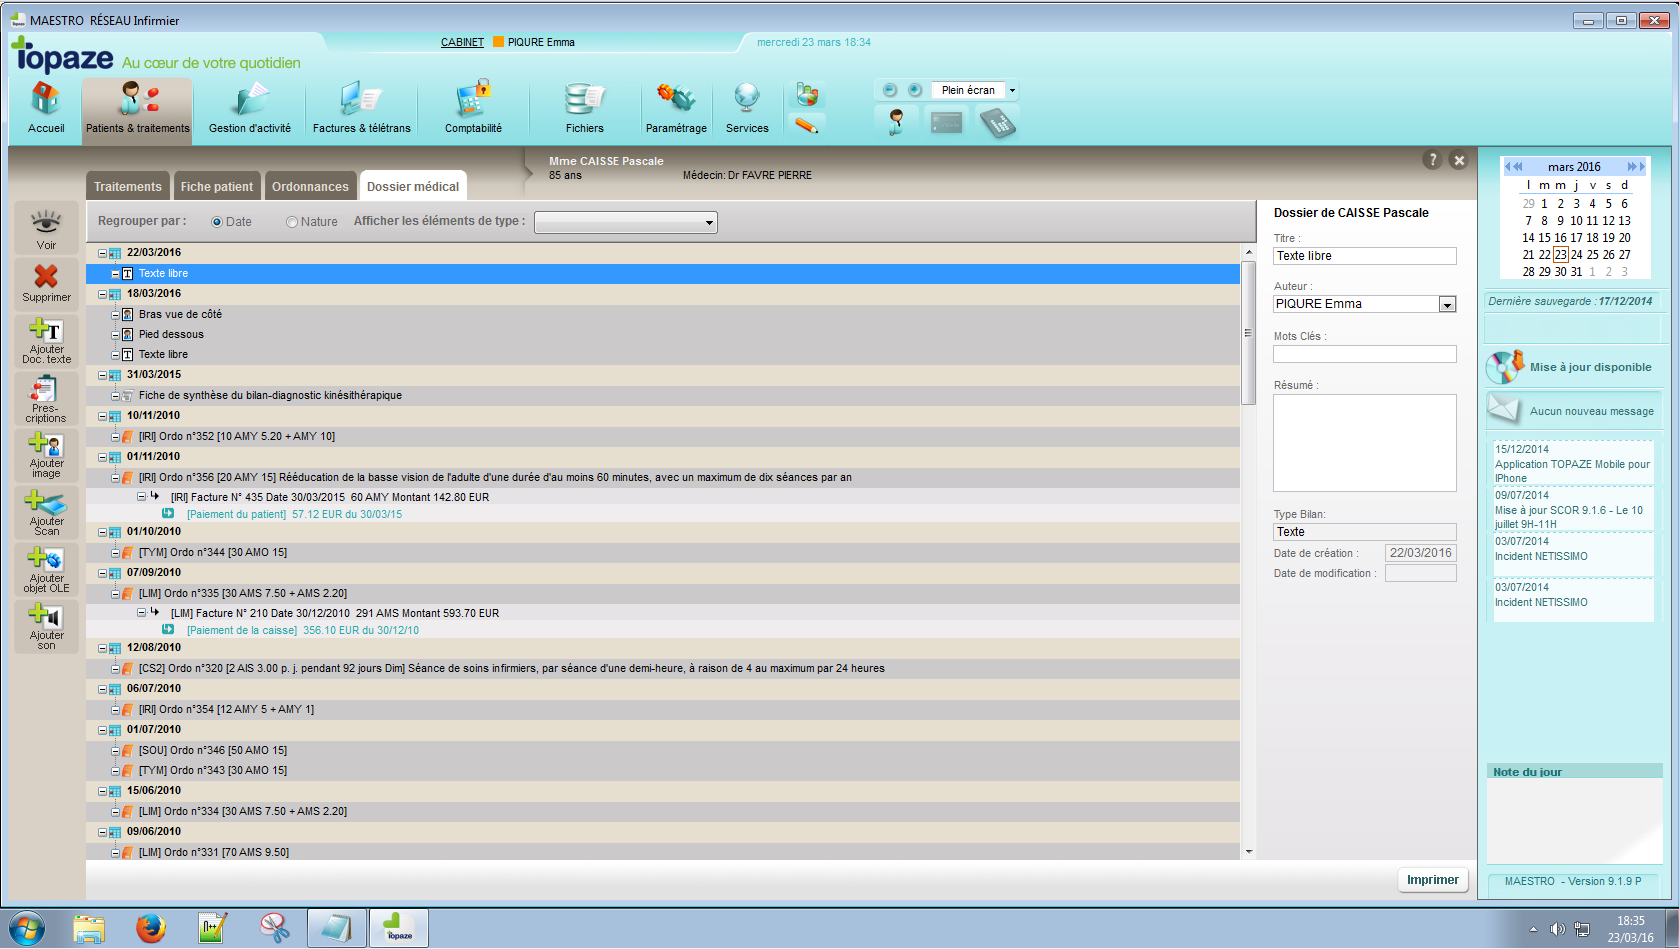
\includegraphics[width=18cm]{./img/medical_data_maestro.PNG}
  \caption{\label{fig:dossier_medical} Dossier médical tel qu'il est présent dans Topaze Maestro.}
\end{figure}

\newpage
\begin{figure}[H]
\section*{L'editeur de texte de Topaze Maestro}
  \centering
  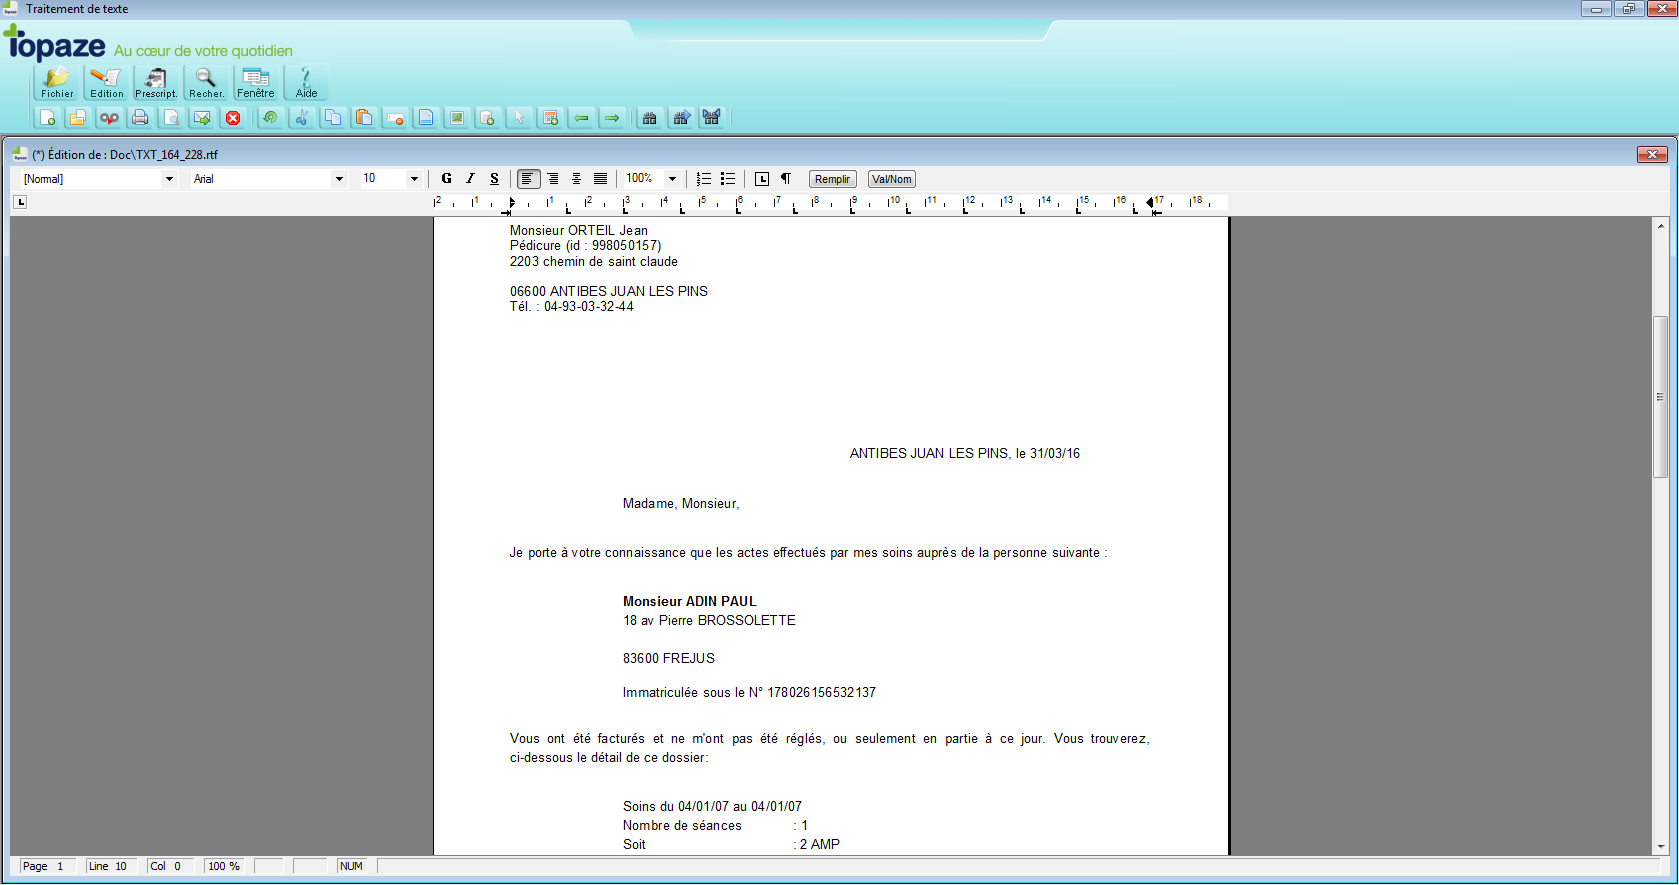
\includegraphics[width=18cm]{./img/text_editor2}
  \caption{\label{fig:editeur_texte} L'éditeur de texte présent dans Topaze Maestro.}
\end{figure}


\newpage
\begin{figure}[H]
\section*{Exemple de modèle XML utilisé par le générateur de code}
  \centering
  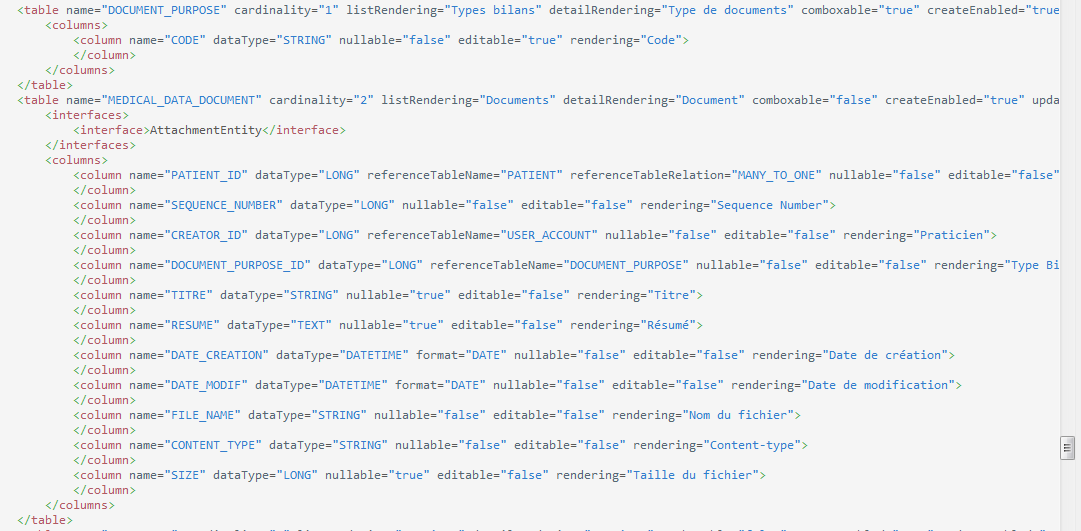
\includegraphics[width=18cm]{./img/modele_generateur}
  \caption{\label{fig:xml} Exemple de modèle décrit en XML à destination du générateur.}
\end{figure}

\begin{figure}[H]
\section*{Diagramme de séquence de la requête d'obtention du dossier médical}
  \centering
  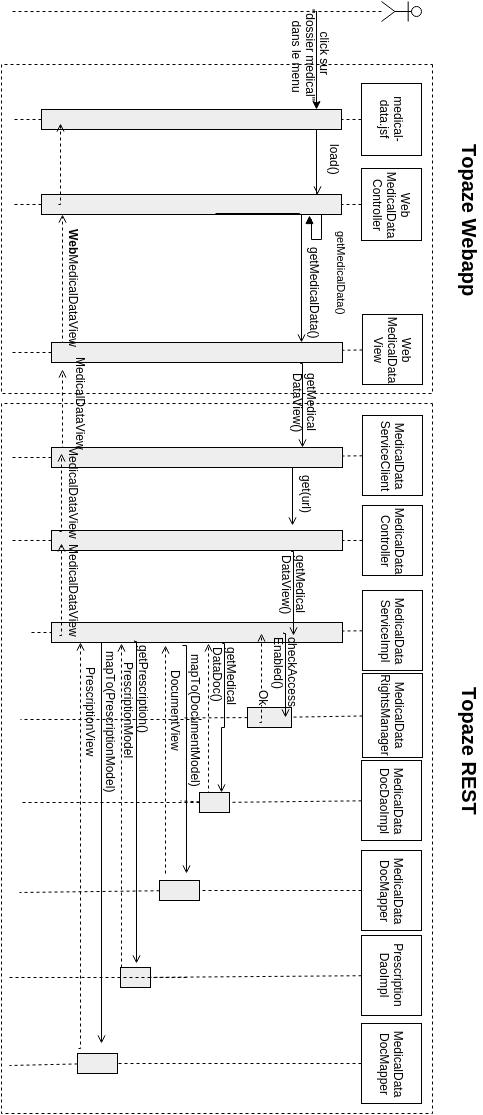
\includegraphics[height=22cm]{./img/diag_seq2}
  \caption{\label{fig:diag_seq} Diagramme de séquence modélisant la requête du dossier médical.}
\end{figure}

\newpage
\begin{figure}[H]
\section*{Le dossier médical de Topaze Web}
  \centering
  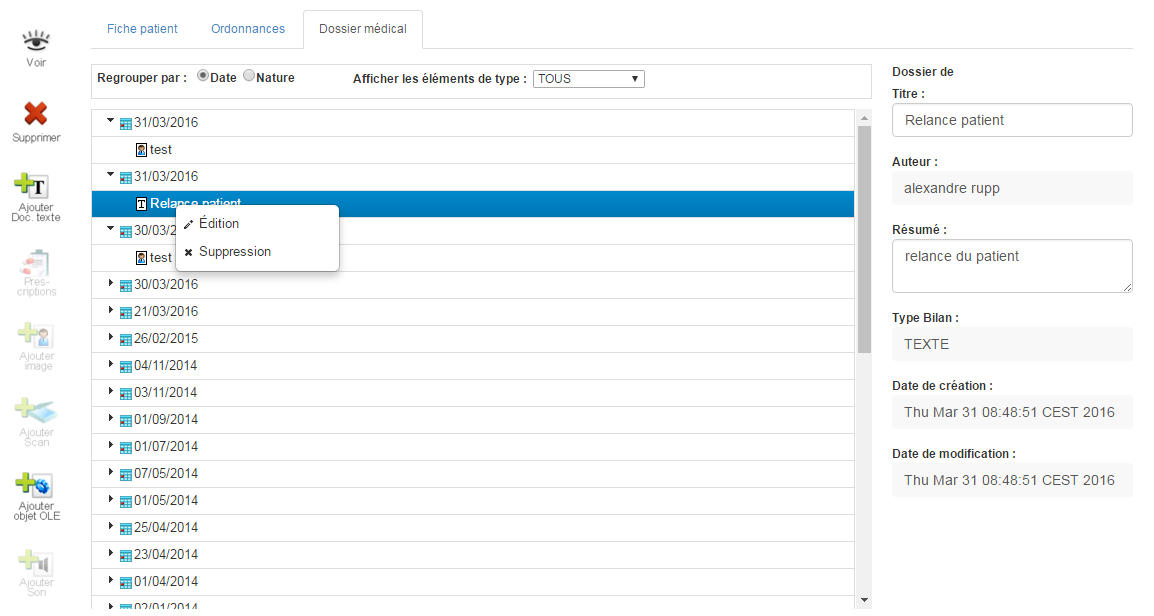
\includegraphics[width=18cm]{./img/dossier_medical_web2}
  \caption{\label{fig:dossier_web} Le dossier médical implémenté dans Topaze Web.}
\end{figure}

\newpage
\begin{figure}[H]
\section*{L'editeur de texte de Topaze Web}
  \centering
  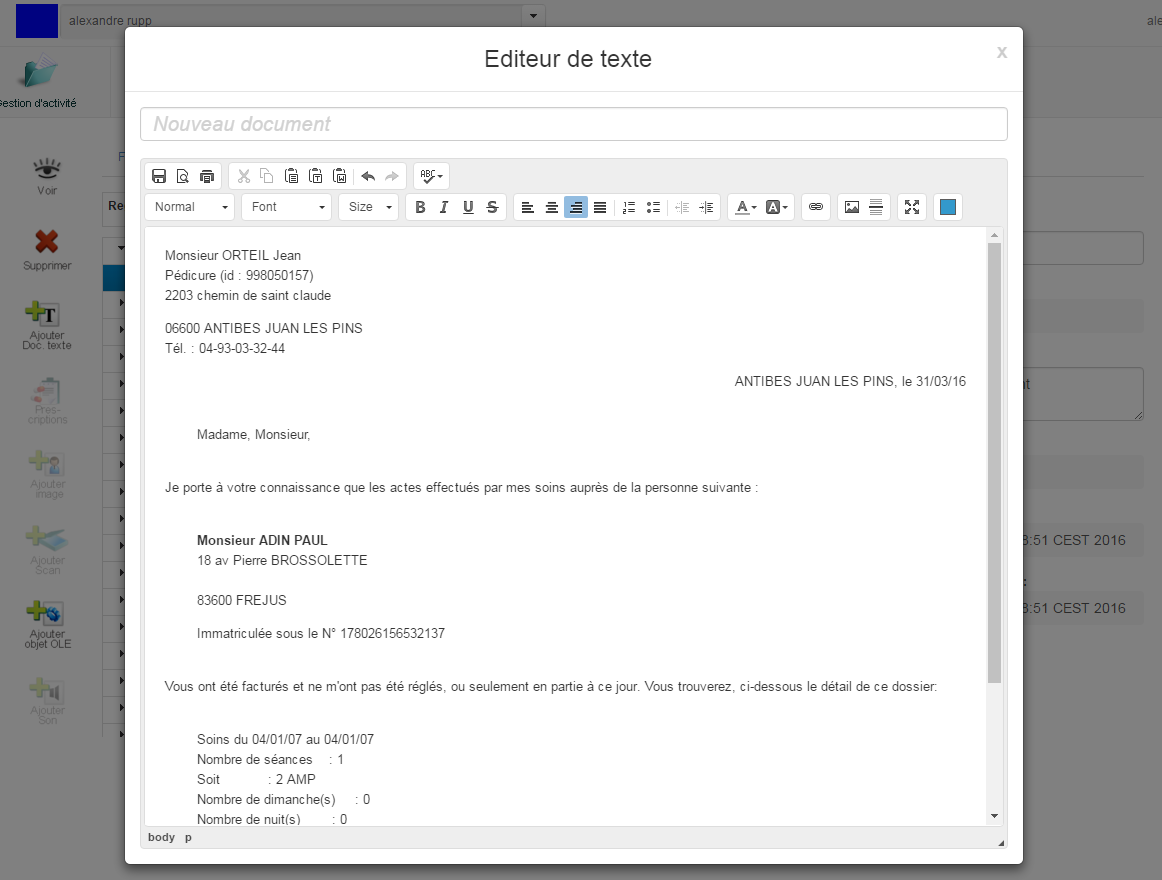
\includegraphics[width=18cm]{./img/editeur_topaze_web}
  \caption{\label{fig:editeur_web} L'éditeur de texte (CKEditor) intégré dans Topaze Web .}
\end{figure}

%\newpage
%\begin{figure}[H]
%\section*{Exemple de classe annotée}
%  \centering
%  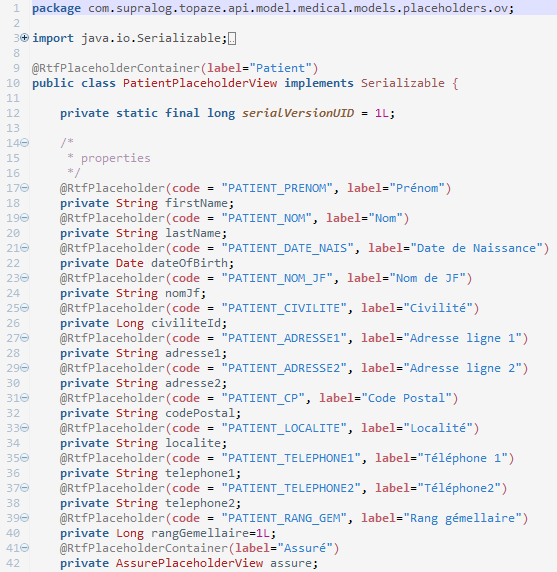
\includegraphics[width=15cm]{./img/annotations}
%  \caption{\label{fig:annotations} La classe Patient a été annotée avec 2 annotations (RtfPlaceholderContainer et RtfPlaceholder) afin de pouvoir être ensuite introspectée et servir à créer l'arborescence de placeholders.}
%\end{figure}

\end{appendices}

 % (0 pages)


\end{document}
